\documentclass[12pt]{article}

% =========================================================================
% Ferrous Bridge --- Synthesis Paper
% Title: "Ferrous Bridge: A C -> Rust Automated Agent Orchestration
%         Pipeline with Type Checks and Safety Guarantees"
% Author: Matthew Long, YonedaAI Research Collective
% Date: 16 April 2026
% =========================================================================

% ----- Fonts and encoding -----
\usepackage[T1]{fontenc}
\usepackage{lmodern}

% ----- Core math -----
\usepackage{amsmath, amssymb, amsthm}
\usepackage{mathtools}

% ----- Inference rules -----
\usepackage{mathpartir}

% ----- Diagrams -----
\usepackage{tikz-cd}
\usepackage{tikz}
\usetikzlibrary{positioning, arrows.meta, shapes.geometric, shapes.misc,
                fit, calc, backgrounds, decorations.pathreplacing, patterns}

% ----- References -----
\usepackage{hyperref}
\usepackage{xurl}
\usepackage{cleveref}
\usepackage{enumitem}

% ----- Page layout -----
\usepackage[margin=1in]{geometry}

% ----- Code listings -----
\usepackage{listings}
\usepackage{xcolor}

% ----- Graphics -----
\usepackage{graphicx}

% ----- Spacing -----
\frenchspacing
\setlength{\emergencystretch}{3em}

% =========================================================================
% Theorem environments
% =========================================================================
\newtheorem{theorem}{Theorem}[section]
\newtheorem{proposition}[theorem]{Proposition}
\newtheorem{lemma}[theorem]{Lemma}
\newtheorem{corollary}[theorem]{Corollary}
\theoremstyle{definition}
\newtheorem{definition}[theorem]{Definition}
\newtheorem{schema}[theorem]{Schema}
\theoremstyle{remark}
\newtheorem{remark}[theorem]{Remark}
\newtheorem{example}[theorem]{Example}

% =========================================================================
% Custom commands --- shared by the synthesis
% =========================================================================
\newcommand{\rust}{\textnormal{\textsc{Rust}}}
\newcommand{\clang}{\textnormal{\textsc{C}}}
\newcommand{\libyaml}{\texttt{libyaml}}
\newcommand{\safelibyaml}{\texttt{safe-libyaml}}
\newcommand{\unsafelibyaml}{\texttt{unsafe-libyaml}}
\newcommand{\libexpat}{\texttt{libexpat}}
\newcommand{\safelibexpat}{\texttt{safe-libexpat}}

% --- Agent / artifact algebra ---
\newcommand{\Agent}[1]{\ensuremath{\mathsf{#1}}}
\newcommand{\Artifact}[1]{\ensuremath{\mathsf{#1}}}
\newcommand{\refines}{\ensuremath{\sqsubseteq}}
\newcommand{\rdef}{\ensuremath{\triangleq}}
\newcommand{\Compile}{\ensuremath{\sqsubseteq_{\!\mathrm{compile}}}}
\newcommand{\Memory}{\ensuremath{\sqsubseteq_{\!\mathrm{mem}}}}
\newcommand{\Behav}{\ensuremath{\sqsubseteq_{\!\mathrm{behav}}}}
\newcommand{\Conc}{\ensuremath{\sqsubseteq_{\!\mathrm{conc}}}}
\newcommand{\Refine}{\ensuremath{\sqsubseteq_{\!\mathrm{ref}}}}
\newcommand{\ABI}{\ensuremath{\sqsubseteq_{\!\mathrm{abi}}}}
\newcommand{\AllRefines}{\ensuremath{\sqsubseteq_{\!\mathrm{full}}}}

% --- Artifact type names ---
\newcommand{\CSrc}{\Artifact{CSource}}
\newcommand{\CAB}{\Artifact{CAB}}
\newcommand{\OSG}{\Artifact{OSG}}
\newcommand{\Scaff}{\Artifact{RustScaffold}}
\newcommand{\RUnit}{\Artifact{RustUnit}}
\newcommand{\BArt}{\Artifact{BuildArtifact}}
\newcommand{\MiriR}{\Artifact{MiriReport}}
\newcommand{\FuzzR}{\Artifact{FuzzReport}}
\newcommand{\KaniP}{\Artifact{KaniProof}}
\newcommand{\ABISig}{\Artifact{ABISignature}}
\newcommand{\BenchR}{\Artifact{BenchReport}}

% --- Common math shortcuts ---
\newcommand{\dom}{\mathrm{dom}}
\newcommand{\codom}{\mathrm{codom}}
\newcommand{\Trace}{\tau}

% =========================================================================
% Listings
% =========================================================================
\definecolor{codegray}{rgb}{0.5,0.5,0.5}
\definecolor{codepurple}{rgb}{0.58,0,0.82}
\definecolor{codegreen}{rgb}{0,0.5,0}
\definecolor{backcolour}{rgb}{0.97,0.97,0.94}
\definecolor{rustbg}{RGB}{248,248,248}

\lstdefinelanguage{Rust}{
  morekeywords={fn,let,mut,pub,struct,enum,impl,trait,for,where,if,else,match,return,
                use,mod,crate,self,Self,as,in,loop,while,break,continue,move,ref,
                unsafe,extern,async,await,dyn,box,type,const,static,super,
                true,false,None,Some,Ok,Err},
  morekeywords=[2]{u8,u16,u32,u64,usize,i8,i16,i32,i64,isize,bool,char,str,String,
                   Vec,VecDeque,Option,Result,Box,Rc,Arc,Cow,HashMap,BTreeMap,
                   Read,Write,Iterator},
  sensitive=true,
  morecomment=[l]{//},
  morecomment=[s]{/*}{*/},
  morestring=[b]",
}
\lstdefinelanguage{Proto}{
  morekeywords={syntax,package,import,message,enum,oneof,repeated,optional,
                required,reserved,bool,bytes,double,float,fixed32,fixed64,
                int32,int64,uint32,uint64,string,sint32,sint64,sfixed32,sfixed64,
                map,returns,service,rpc,extend,extensions,group},
  sensitive=true,
  morecomment=[l]{//},
  morecomment=[s]{/*}{*/},
  morestring=[b]",
}
\lstdefinestyle{cstyle}{
  language=C,
  backgroundcolor=\color{backcolour},
  commentstyle=\color{codegreen},
  keywordstyle=\color{codepurple},
  basicstyle=\ttfamily\footnotesize,
  breaklines=true,
  showstringspaces=false,
  frame=single,
  framerule=0.3pt,
  rulecolor=\color{gray!50},
  xleftmargin=4pt,
  xrightmargin=4pt
}
\lstdefinestyle{ruststyle}{
  language=Rust,
  backgroundcolor=\color{rustbg},
  commentstyle=\color{codegreen},
  keywordstyle=\color{codepurple},
  basicstyle=\ttfamily\footnotesize,
  breaklines=true,
  showstringspaces=false,
  frame=single,
  framerule=0.3pt,
  rulecolor=\color{gray!50},
  xleftmargin=4pt,
  xrightmargin=4pt
}
\lstdefinestyle{protostyle}{
  language=Proto,
  backgroundcolor=\color{backcolour},
  commentstyle=\color{codegreen},
  keywordstyle=\color{codepurple},
  basicstyle=\ttfamily\footnotesize,
  breaklines=true,
  showstringspaces=false,
  frame=single,
  framerule=0.3pt,
  rulecolor=\color{gray!50},
  xleftmargin=4pt,
  xrightmargin=4pt
}
\lstdefinestyle{bashstyle}{
  language=bash,
  backgroundcolor=\color{backcolour},
  commentstyle=\color{codegreen},
  keywordstyle=\color{codepurple},
  basicstyle=\ttfamily\footnotesize,
  breaklines=true,
  showstringspaces=false,
  frame=single,
  framerule=0.3pt,
  rulecolor=\color{gray!50},
  xleftmargin=4pt,
  xrightmargin=4pt
}

% =========================================================================
% Task-list environment for the dev plan
% =========================================================================
\newenvironment{tasklist}{%
  \begingroup\raggedright
  \begin{description}[style=nextline, leftmargin=1.4cm, itemsep=0.4em]
}{%
  \end{description}
  \endgroup
}

% =========================================================================
% GrokRxiv sidebar (page 1 only)
% =========================================================================
\definecolor{grokgray}{RGB}{110,110,110}
\AddToHook{shipout/foreground}{%
  \ifnum\value{page}=1
    \begin{tikzpicture}[remember picture, overlay]
      \node[
        rotate=90,
        anchor=south,
        font=\Large\sffamily\bfseries\color{grokgray},
        inner sep=0pt
      ] at ([xshift=38pt, yshift=0.52\paperheight]current page.south west)
      {GrokRxiv:2026.04.synthesis\quad
       [\,cs.PL\,]\quad
       16 Apr 2026};
    \end{tikzpicture}
  \fi
}

% =========================================================================
% Title block
% =========================================================================
\title{Ferrous Bridge: A C\,$\to$\,Rust Automated Agent Orchestration Pipeline\\
with Type Checks and Safety Guarantees\\[0.5em]
\large A Synthesis of the \texttt{c}, \texttt{rust}, and
\texttt{c-rust-transpiling} Companion Papers}

\author{Matthew Long\\
\textit{The YonedaAI Collaboration, YonedaAI Research Collective}\\
Chicago, IL\\
\texttt{matthew@yonedaai.com} $\cdot$ \url{https://yonedaai.com}}

\date{16 April 2026}

\begin{document}
\maketitle

\begin{abstract}
The Ferrous Bridge programme has produced three companion technical papers:
Part~I (\emph{The C Language as a Translation Source}) characterises the
implicit invariants encoded in idiomatic C; Part~II (\emph{Idiomatic Safe
Rust as a Translation Target}) characterises the explicit invariants the
target crate must enforce; and Part~III (\emph{Automated C\,$\to$\,Rust
Transpiling}) characterises the per-stage refactoring engine that walks
each function up the safety ladder. None of the three, taken alone, is
itself a build-system. This paper closes the gap. We frame Ferrous Bridge
as a \emph{multi-agent orchestration pipeline}: a typed directed acyclic
workflow whose nodes are AI-driven (or human-supervised) agents and whose
edges carry typed artifacts. Pipeline composition is the orchestration
analogue of \texttt{rustc}'s type system: an upstream agent's output
schema must unify with the downstream agent's input schema, and the
Claude Code subagent supervisor refuses to run a stage whose input fails schema
validation. We give a formal account of (i) the artifact-type category
(eleven artifact types, ten agents, one DAG, one supervisor channel),
(ii) the six-rung safety ladder ($\Compile$, $\Memory$, $\Behav$,
$\Conc$, $\Refine$, $\ABI$) as a chain of refinement relations, and
(iii) an informal composition theorem stating that if every agent
satisfies its rung the resulting \safelibyaml{} crate is observationally
equivalent to \libyaml{} modulo allocator choice and is free of every
undefined-behaviour class enumerated in Part~I. We instantiate the
pipeline on \libyaml{} (the one-week proof) and on \libexpat{} (the
second instance, demonstrating library-agnosticism). Appendix~A is a
38-task development plan for the orchestration layer itself --- the
Claude Code subagent supervisor, the protobuf artifact schemas, the typed message bus,
the workflow DAG executor, the telemetry surface, and the end-to-end
\texttt{ferrous-bridge run} CLI --- granular enough that a reader can
fork the prototype today and execute it.
\end{abstract}

\tableofcontents
\newpage

% =========================================================================
\section{Introduction}
\label{sec:intro}
% =========================================================================

\subsection{The problem}
\label{sec:problem}

C is the dominant systems-software substrate. Approximately thirty
billion lines of C and C++ run the kernels, network stacks, parsers,
codecs, and cryptography of every connected device on the planet. A
disproportionate share of the exploitable vulnerability landscape
inheres in this substrate: the National Vulnerability Database has
catalogued more than two thousand five hundred memory-safety CVEs whose
root cause is unchecked pointer arithmetic, use-after-free, or a buffer
overrun. Each individual CVE is a violation of an invariant the
programmer held in their head but the C compiler did not check.
Part~I, \S{}3 enumerates seven canonical classes of these invariants
(spatial safety, temporal safety, type-based aliasing, signed overflow,
unsequenced modification, indeterminate values, concurrent races) and
shows, class by class, that each is forbidden by an explicit feature of
\rust{}'s type system.

The naive response --- \emph{rewrite it all in Rust by hand} --- does
not scale. Manual rewrites of high-assurance C consume between four and
one hundred fifty engineer-dollars per line~\cite{economics2026}. The
collected memory-safe-language replacements shipped by Prossimo and
Trifecta over the last five years (\texttt{rustls}, \texttt{sudo-rs},
\texttt{ntpd-rs}, Hickory~DNS, \texttt{rav1d}, \texttt{zlib-rs},
\texttt{libbzip2-rs}) consumed thousands of senior-engineer hours each.
At the prevailing rate of human throughput the global addressable C
codebase will not be migrated this century.

The mechanical response --- \emph{transpile it with c2rust} --- also
does not scale, but for a different reason. Immunant's c2rust toolchain
is the canonical AST-level transpiler and the foundation of the
\unsafelibyaml{} crate that backs ninety million transitive downloads of
\texttt{serde\_yaml} and its forks. But c2rust, as Part~III, \S{}2.1
documents, produces \emph{pervasively-\texttt{unsafe}} \rust{}: it
preserves the original C control flow, the raw pointer arithmetic, and
the error-code returns. The result compiles under \texttt{rustc} and
runs at C-equivalent speed but provides essentially zero security value;
the implicit invariants of the original C remain implicit in the output
\rust{}, now wrapped in \texttt{unsafe} blocks instead of unstated
assumptions.

The interesting middle ground --- \emph{LLM-assisted, formally-verified,
agent-orchestrated translation} --- has been discussed in the literature
since SACTOR~\cite{sactor2025} and ForCLift but has not, prior to the
present work, been delivered as an end-to-end build-system that takes
\(\langle\)~C source repository~\(\rangle\) on standard input and emits
\(\langle\)~safe Rust crate that compiles, passes Miri, survives a
million fuzz inputs, and proves the chosen invariants in
Kani~\(\rangle\) on standard output. That is the gap Ferrous Bridge
fills.

\subsection{The thesis}
\label{sec:thesis}

The synthesis thesis of this paper has three components.

\paragraph{Thesis 1: orchestration is a typing problem.}
The conventional framing of multi-agent AI systems is operational:
agents are coroutines that swap messages on a queue, the supervisor is a
scheduler, and correctness is checked end-to-end after the workflow
finishes. We argue that this framing is exactly inverted for
high-assurance translation. Each pipeline stage is a \emph{morphism}
\(\Agent{A}_i : \Artifact{In}_i \to \Artifact{Out}_i\) between
artifact types, the supervisor is a \emph{type-checker}, and pipeline
composition is well-typed if and only if
\(\Artifact{Out}_i = \Artifact{In}_{i+1}\). This is the same discipline
\rust{} imposes on a function call. Section~\ref{sec:dag} formalises
it.

\paragraph{Thesis 2: safety is a refinement chain.}
The six rungs of the safety ladder ---
$\Compile$, $\Memory$, $\Behav$, $\Conc$, $\Refine$, $\ABI$ --- are
refinement relations on the artifact \safelibyaml{} considered as a
candidate for libyaml. A pipeline run that produces an artifact
satisfying all six rungs has, in a precise sense
(Theorem~\ref{thm:composition}), discharged every undefined-behaviour
class enumerated in Part~I, \S{}3 and exposed every API surface
required by the C consumers enumerated in Part~II, \S{}9. Each rung
corresponds to a specific verifier: \texttt{rustc -D warnings},
\texttt{cargo +nightly miri test}, the differential fuzz harness,
\texttt{cargo careful test} plus Loom, \texttt{cargo kani}, and
\texttt{cbindgen} diff against the original \texttt{yaml.h}. The
informal composition theorem of \S{}\ref{sec:composition} says that
the chain composes monotonically: an artifact rejected at rung \(k\)
cannot satisfy rungs \(k+1\) through \(6\), so the pipeline can stop
early on the first failed rung and ship a structured
\texttt{Err(...)} report rather than a silently-wrong crate.

\paragraph{Thesis 3: the orchestration generalises across
streaming-parser libraries.} The DAG of \S{}\ref{sec:dag},
instantiated against \libyaml{}, produces \safelibyaml{} in seven
working days at a Claude API cost of \$85--\$240. The \emph{same}
DAG, with the same agents and the same schemas, instantiated against
\libexpat{} produces \safelibexpat{} in eight to ten working days; the
only differences are SAX-style callbacks (closures replace function
pointers), entity-expansion recursion limits (an additional Kani
target), and namespace separator validation (a constructor-time
precondition). We emphasise that the two demonstrated targets are
both streaming parsers with similar structural properties (tokenise,
state-machine, emit events); we do \emph{not} claim that the same
phase-B decomposition applies unchanged to a cryptography library, a
scientific-computing kernel, a compression codec, or a database
engine. Section~\ref{sec:libexpat} re-instantiates the pipeline
against \libexpat{} and \S{}\ref{sec:libexpat-limits} discusses the
open question of how far beyond streaming parsers the decomposition
extends.

\subsection{Roadmap}
\label{sec:roadmap}

The paper is structured as follows.
Section~\ref{sec:partsoverview} summarises the three companion papers
and their cross-cutting themes.
Section~\ref{sec:dag} formalises the orchestration pipeline as a typed
directed acyclic workflow.
Section~\ref{sec:safety-ladder} formalises the six-rung safety ladder
as a chain of refinement relations.
Section~\ref{sec:composition} states the (informal) composition
theorem.
Section~\ref{sec:typecheck} treats the per-hand-off type check, the
protobuf schemas, and the supervisor's schema-validation step.
Section~\ref{sec:libyaml} relates the day-by-day \libyaml{} schedule of
Part~III, \S{}9 to the agents and ladder rungs of this paper.
Section~\ref{sec:libexpat} re-instantiates the DAG against \libexpat{}
and identifies what changes and what does not.
Section~\ref{sec:emergent} discusses emergent properties of the
composition: bounded human-review escalation, the training-data harvest,
the fine-tuned-model feedback loop, and the cost trajectory.
Section~\ref{sec:related} surveys related work.
Section~\ref{sec:conclusion} closes.
Appendix~\ref{app:devplan} is the orchestration-layer development plan.

% =========================================================================
\section{The Three Companion Papers as Parts I, II, and III}
\label{sec:partsoverview}
% =========================================================================

We refer to the three companion papers as \textbf{Part~I}
\cite{long-c}, \textbf{Part~II} \cite{long-rust}, and \textbf{Part~III}
\cite{long-transpile}. Their roles in the synthesis are complementary
and asymmetric: Part~I is a \emph{theory of the source}, Part~II is a
\emph{theory of the target}, and Part~III is a \emph{theory of the
process}. The synthesis presented here is the \emph{theory of the
build-system} that wires the three together. We summarise each Part and
then enumerate the cross-cutting themes that make their composition
non-trivial.

\subsection{Part~I --- The C Language as a Translation Source}

Part~I gives a small-step operational semantics for a translation-relevant
fragment of C, organises the standard's undefined behaviour into seven
classes (UB1--UB7), catalogues the eleven recurring \clang{} idioms found
in \libyaml{}, and discharges, for each idiom, a \emph{translation
contract}: a typed refinement statement plus its proof obligation. The
key technical artifacts of Part~I are:

\begin{itemize}
\item \textbf{Theorem~3.2} (Part~I, \S{}3) --- a seven-class UB
taxonomy mapping each undefined-behaviour class to the precise \rust{}
type-system feature that statically forbids it.
\item \textbf{Idioms I1--I11} (Part~I, \S{}4) --- the
\texttt{yaml\_string\_t} triple, the \texttt{STACK\_*}/\texttt{QUEUE\_*}/
\texttt{STRING\_*} macro families, the integer-as-bool return
convention, the tagged-union event type, the custom allocator hooks,
the scanner-into-parser buffer aliasing, nullable optional pointers, the
ambient parser-resident error field, character-predicate macros, the
output-parameter convention, and \texttt{setjmp}/\texttt{longjmp} as the
limit case.
\item \textbf{Translation contracts (Definition~5.1)} --- the typed
refinement statements that say, of each idiom, ``if these side
conditions are discharged then the corresponding \rust{} construct is a
faithful refinement.''
\end{itemize}

In the synthesis these artifacts feed Stage~2 (Ownership Semantic
Graph) and Stage~3 (Translation Engine): a contract is the rule against
which the OSG-builder annotates each pointer parameter, and the
discharge of the contract's proof obligation is the success criterion of
the translation step.

\subsection{Part~II --- Idiomatic Safe Rust as a Translation Target}

Part~II is a design specification for \safelibyaml{}: it characterises
\emph{what idiomatic safe \rust{} should look like} for a streaming
parser library and what engineering rules a translation pipeline must
follow to hit that target deterministically. Its key technical artifacts:

\begin{itemize}
\item \textbf{Definition~1.1--1.3} (Part~II, \S{}1) --- the
operational definitions of \emph{safe}, \emph{idiomatic}, and
\emph{ABI-compatible} \rust{}: zero \texttt{unsafe} outside the FFI
shim, Miri-clean, \texttt{Result<T,E>} everywhere, \texttt{Option<T>}
everywhere, \texttt{enum} for every tagged union, iterator adapters
where C uses index loops, and a \texttt{cbindgen}-diff-empty FFI header
matching \texttt{yaml.h} byte-for-byte.
\item \textbf{Section~4} --- the lifetime-parameterised
\texttt{Event<\textbackslash 'a>} enum with \texttt{Cow<\textbackslash 'a, str>} payloads, the
solution to the self-referential emitter problem (the
\texttt{Analysis<\textbackslash 'a>} lifetime that carries the
borrow from the event being analysed).
\item \textbf{Section~5} --- the \texttt{thiserror}-derived
structured \texttt{Error} type matching libyaml's existing problem
categories.
\item \textbf{Sections~7--8} --- the strict no-\texttt{unsafe} core
paired with a thin \texttt{extern "C"} ABI shim
\texttt{safe-libyaml-sys}, exporting the symbol set required by
\texttt{serde\_yaml\_ng} and \texttt{serde\_yaml\_bw}.
\end{itemize}

In the synthesis these artifacts feed Stage~3 (Translation Engine) and
Stage~4 (Verification Pipeline): the design rules are the prompts that
constrain the translation, and the \texttt{cbindgen}-diff is rung
\(\ABI\) of the safety ladder.

\subsection{Part~III --- Automated C\,$\to$\,Rust Transpiling}

Part~III treats the \emph{process}: how to take a C source file and
walk it up the safety ladder one refactoring step at a time. Its key
technical artifacts:

\begin{itemize}
\item \textbf{Lemma~5.1} (Part~III, \S{}5) --- the
refactoring-soundness lemma: each of the twelve refactor patterns
(raw-pointer dereference $\to$ slice indexing, \texttt{strcmp == 0}
$\to$ \texttt{==}, tagged union $\to$ \texttt{enum}, etc.) preserves
observable behaviour modulo a side condition that the OSG provides.
\item \textbf{Section~7} --- the differential-fuzz harness: take an
input, run \libyaml{} and \safelibyaml{} on it, compare the event
streams, declare divergence on first mismatch.
\item \textbf{Section~8} --- the Miri / Kani / Loom /
\texttt{cargo-careful} ladder of dynamic-analysis tooling.
\item \textbf{Appendix~A} (Part~III, \S{}10) --- the day-by-day
seven-day \libyaml{} schedule that we re-frame in
\Cref{sec:libyaml}.
\end{itemize}

In the synthesis these feed Stage~3, Stage~4, and the \libyaml{}
proof of \Cref{sec:libyaml}.

\subsection{Cross-cutting themes}
\label{sec:crosscutting}

The three Parts intersect at four points; the synthesis exists to make
those intersections explicit. We illustrate each by citing the precise
result from each Part.

\paragraph{Theme~1: UB taxonomy $\leftrightarrow$ Rust feature
$\leftrightarrow$ refactor pattern.} Each entry in the seven-class UB
taxonomy of Part~I, \S{}3 has a counterpart in Part~II's design rules
(the precise \rust{} feature that forbids it) and a counterpart in
Part~III's twelve refactor patterns (the mechanical rewrite that climbs
from \unsafelibyaml{} to \safelibyaml{}). Concretely, UB1 (spatial
memory safety) of Part~I, \S{}3.1 is forbidden by checked slice
indexing of Part~II, \S{}3.2 and is climbed by refactor pattern~1 of
Part~III, \S{}5.1 (\texttt{*ptr} $\Rightarrow$ \texttt{buf[i]}). The
chain
\[
\text{Theorem~3.2 of Part~I (UB taxonomy)}
\;\longleftrightarrow\;
\text{Section~4 of Part~II (matched Rust feature)}
\;\longleftrightarrow\;
\text{Lemma~5.1 of Part~III (refactor soundness)}
\]
underlies every line of \safelibyaml{}: each refactored line has a UB
class it discharges, a Rust feature that does the discharging, and a
refactor pattern that performed the discharge.

\paragraph{Theme~2: idiom $\leftrightarrow$ design rule
$\leftrightarrow$ translation step.} Part~I's eleven idioms (\S{}4),
Part~II's design rules (\S{}\S{}3--8), and Part~III's per-day
schedule (\S{}9) are aligned. Idiom~I8 of Part~I (the tagged-union
\texttt{yaml\_event\_t}) is met by Part~II's
\texttt{Event<\textbackslash 'a>} enum (\S{}4) and is translated on
Day~2 of Part~III's schedule by agent~B2 (\S{}9.2 of Part~III). The
synthesis pipeline selects which idiom each agent must handle.

\paragraph{Theme~3: contract $\leftrightarrow$ verifier
$\leftrightarrow$ ladder rung.} Each of Part~I's translation contracts
(\S{}5) requires discharge of a proof obligation. The proof
obligations are checked by Part~III's verifiers (\S{}\S{}7--8). The
verifiers in turn implement the rungs of \S{}\ref{sec:safety-ladder}
of the present paper. \texttt{rustc -D warnings} discharges the
``compiles'' obligation; Miri discharges the ``no UB at run time''
obligation; differential fuzz discharges the ``observably equivalent''
obligation. The synthesis composes the verifiers into the safety
ladder.

\paragraph{Theme~4: \libyaml{} $\to$ \libexpat{}.} Part~I, Part~II,
and Part~III all argue that the \libyaml{} pipeline generalises:
Part~I, \S{}4 catalogues the idioms by archetype, not by library;
Part~II, \S{}10 sketches the \libexpat{} API; Part~III, \S{}11 lists
what changes (callbacks, entity-expansion limits, namespace separators)
and what does not (the safety ladder, the differential-fuzz harness,
the Miri gate, the entire 12-pattern refactoring catalogue). The
synthesis pipeline of \Cref{sec:dag} is the formal artefact that
embodies this generalisation: the DAG is library-agnostic; the seed
corpus and the type contracts in \texttt{src/types/} are
library-specific.

% =========================================================================
\section{The Orchestration Pipeline as a Typed DAG}
\label{sec:dag}
% =========================================================================

\subsection{Agents as morphisms; artifacts as types}
\label{sec:morphisms}

We give a \emph{type-system-inspired} presentation that, while it
borrows category-theoretic vocabulary, makes no claim to be a formal
category in the strict sense. The presentation lets us state the
type-checking obligation precisely; the categorical language is
notational scaffolding rather than load-bearing structure.

\begin{definition}[Artifact type system]
\label{def:artifact-cat}
The \emph{artifact type system} consists of (i) the artifact types
listed in \Cref{tab:artifact-types}, regarded as syntactic tags, and
(ii) a collection of \emph{agents} \(\Agent{A} : X \to Y\), each of
which consumes an artifact of type \(X\) and emits an artifact of type
\(Y\). We use the symbol \(\circ\) for sequential agent execution
(\(\Agent{B} \circ \Agent{A}\) means ``run \(\Agent{A}\) first, then
\(\Agent{B}\) on the result''), and \(\mathrm{id}_X\) for the trivial
pass-through agent on type \(X\). We do \emph{not} claim that this
forms a category in the strict mathematical sense; in particular, we
make no claim about associativity coherence or the existence of
identities for every type. The vocabulary is borrowed for clarity.
\end{definition}

\begin{table}[h]
\centering
\small
\begin{tabular}{|l|l|l|}
\hline
\textbf{Type} & \textbf{Schema} & \textbf{Description}\\
\hline
\CSrc & \texttt{c\_source.proto} & C source file plus build system metadata\\
\CAB & \texttt{cab.proto} & C-Analysis Bundle: AST, CFG, call graph, points-to, traces\\
\OSG & \texttt{osg.proto} & Ownership Semantic Graph: per-pointer ownership class\\
\Scaff & \texttt{scaffold.proto} & Empty-bodied Rust crate with type definitions\\
\RUnit & \texttt{rust\_unit.proto} & Translated Rust function or module body\\
\BArt & \texttt{build\_artifact.proto} & Compiled \texttt{cargo} target with metadata\\
\MiriR & \texttt{miri\_report.proto} & Miri test results and UB diagnostics\\
\FuzzR & \texttt{fuzz\_report.proto} & cargo-fuzz / AFL++ campaign results\\
\KaniP & \texttt{kani\_proof.proto} & Kani harness verdict per critical function\\
\ABISig & \texttt{abi\_signature.proto} & cbindgen-emitted C header signature\\
\BenchR & \texttt{bench\_report.proto} & criterion benchmark results vs C reference\\
\hline
\end{tabular}
\caption{The eleven artifact types of the Ferrous Bridge orchestration
pipeline. Each has a protobuf schema (Section~\ref{sec:typecheck})
against which the supervisor validates inputs and outputs.}
\label{tab:artifact-types}
\end{table}

\begin{definition}[Composition]
\label{def:composition}
Two agents \(\Agent{A} : X \to Y\) and \(\Agent{B} : Y' \to Z\) compose
to \(\Agent{B} \circ \Agent{A} : X \to Z\) if and only if \(Y = Y'\).
The supervisor (orchestrated via Claude Code subagents; \S{}\ref{sec:typecheck}) refuses to schedule
\(\Agent{B}\) on the output of \(\Agent{A}\) when this equation fails,
emitting a structured \texttt{SchemaMismatch} error to the
human-review queue.
\end{definition}

This is the orchestration analogue of the \rust{} type rule for
function calls: \(f : X \to Y\) and \(g : Y' \to Z\) compose if
\(Y = Y'\), and the type-checker rejects programs where the equation
fails. We exploit this analogy throughout: the orchestration pipeline
\emph{is} a \rust{} program in which agents are functions, the
artifact category provides the types, and the Claude Code subagent supervisor is
\texttt{rustc}.

\subsection{The ten agents and the workflow DAG}
\label{sec:ten-agents}

The Ferrous Bridge pipeline factors into ten agents grouped into three
phases (A, B, C) plus the supervisor channel. We list them in
\Cref{tab:agents} and draw their composition in \Cref{fig:dag}.

\begin{table}[h]
\centering
\small
\begin{tabular}{|l|l|l|l|l|}
\hline
\textbf{Agent} & \textbf{Phase} & \textbf{Mission} & \textbf{Input} & \textbf{Output}\\
\hline
\(\Agent{A}_1\) & A & Source Analyst & \CSrc & \CAB\\
\(\Agent{A}_2\) & A & Scaffold Builder & \CAB & \Scaff\\
\(\Agent{A}_3\) & A & Test Harness Builder & \CSrc{} + \Scaff & \BArt\\
\(\Agent{B}_1\) & B & Reader/Writer Translator & \OSG{} + \Scaff & \RUnit\\
\(\Agent{B}_2\) & B & API Layer Translator & \OSG{} + \Scaff & \RUnit\\
\(\Agent{B}_3\) & B & Parser Translator & \OSG{} + \Scaff & \RUnit\\
\(\Agent{B}_4\) & B & Scanner Translator & \OSG{} + \Scaff & \RUnit\\
\(\Agent{B}_5\) & B & Emitter Translator & \OSG{} + \Scaff & \RUnit\\
\(\Agent{C}_1\) & C & Compiler Fixer & \(\bigsqcup_i \RUnit\) & \BArt\\
\(\Agent{C}_2\) & C & Safety Auditor & \BArt & \MiriR\\
\(\Agent{C}_3\) & C & Equivalence Tester & \BArt & \FuzzR\\
\(\Agent{C}_4\) & C & Idiom Polisher & \(\bigsqcup_i \RUnit\) & \(\bigsqcup_i \RUnit\)\\
\(\Agent{C}_5\) & C & Benchmarker & \BArt & \BenchR\\
\(\Agent{K}\)   & C & Kani Prover & \BArt & \KaniP\\
\(\Agent{F}\)   & C & ABI Shim Builder & \BArt & \ABISig\\
\(\Agent{R}\)   & * & Subagent Supervisor & all & escalation queue\\
\hline
\end{tabular}
\caption{The agents of the Ferrous Bridge pipeline, their input and
output artifact types, and their phase. \(\bigsqcup\) denotes the
disjoint sum (multi-input) of \RUnit{} artifacts assembled by the
compiler-fixer and idiom-polisher.}
\label{tab:agents}
\end{table}

The OSG (\OSG) is built from the CAB (\CAB) by a deterministic ownership
classifier; we treat the classifier as a sub-agent of \(\Agent{A}_1\)
for purposes of the synthesis paper, in keeping with Part~I,
\S{}1.1.

\begin{figure}[t]
\centering
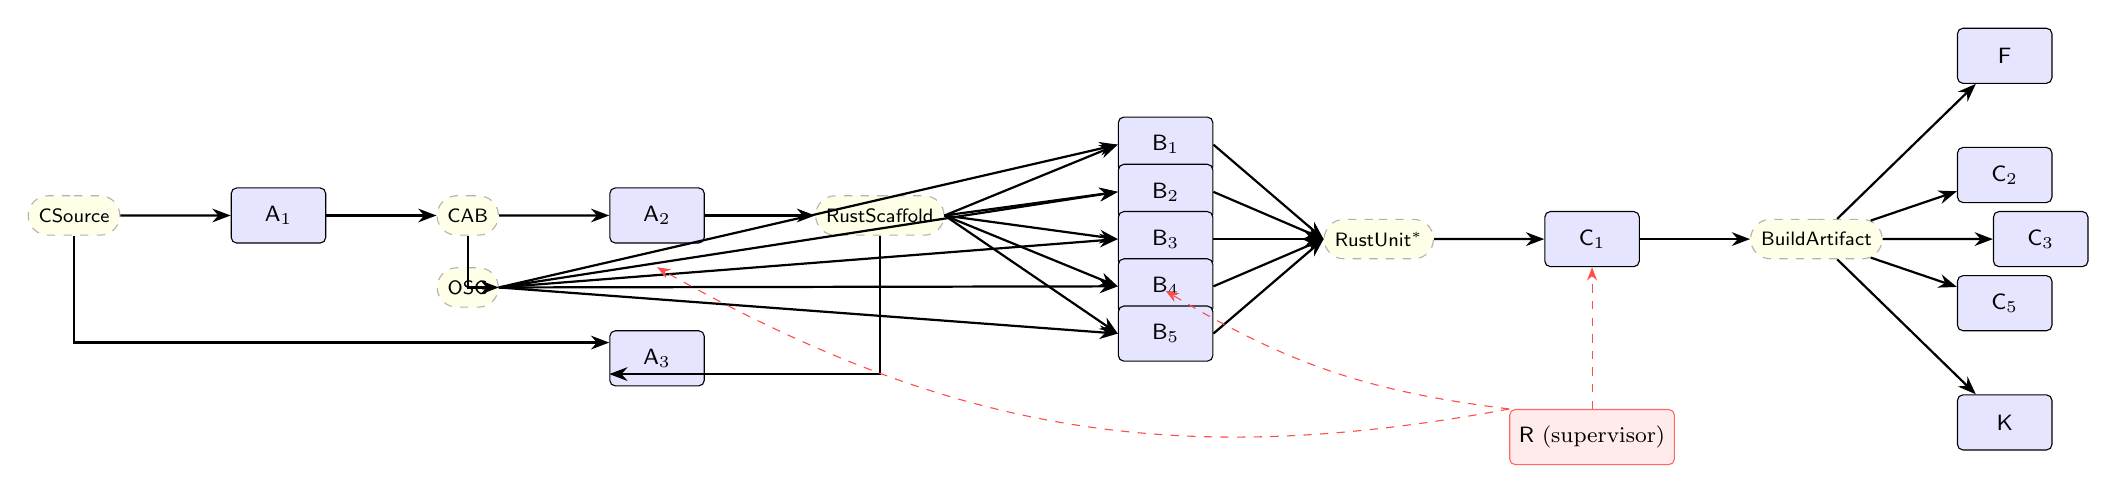
\begin{tikzpicture}[
  node distance=11mm and 14mm,
  every node/.style={font=\footnotesize},
  agent/.style={draw, rounded corners=2pt, minimum height=7mm, minimum width=12mm,
                fill=blue!10},
  artifact/.style={draw=gray!60, dashed, rounded rectangle, minimum height=5mm,
                   font=\scriptsize\itshape, fill=yellow!10},
  super/.style={draw=red!60, fill=red!8, rounded corners=2pt, minimum height=7mm,
                minimum width=12mm},
  arr/.style={->, >=Stealth, thick}
]
% inputs
\node[artifact] (csrc) {\CSrc};
\node[agent, right=of csrc] (a1) {$\Agent{A}_1$};
\node[artifact, right=of a1] (cab) {\CAB};
\node[artifact, below=4mm of cab] (osg) {\OSG};

\node[agent, right=of cab] (a2) {$\Agent{A}_2$};
\node[artifact, right=of a2] (sc) {\Scaff};

\node[agent, below=of a2] (a3) {$\Agent{A}_3$};

% B agents (translators)
\node[agent, right=22mm of sc, yshift= 9mm] (b1) {$\Agent{B}_1$};
\node[agent, right=22mm of sc, yshift= 3mm] (b2) {$\Agent{B}_2$};
\node[agent, right=22mm of sc, yshift=-3mm] (b3) {$\Agent{B}_3$};
\node[agent, right=22mm of sc, yshift=-9mm] (b4) {$\Agent{B}_4$};
\node[agent, right=22mm of sc, yshift=-15mm] (b5) {$\Agent{B}_5$};

\node[artifact, right=14mm of b3] (rus) {\RUnit{}\(^*\)};

\node[agent, right=of rus] (c1) {$\Agent{C}_1$};
\node[artifact, right=of c1] (ba) {\BArt};

% C verifiers
\node[agent, above right=2mm and 12mm of ba] (c2) {$\Agent{C}_2$};
\node[agent, right=14mm of ba]                 (c3) {$\Agent{C}_3$};
\node[agent, below right=2mm and 12mm of ba]   (c5) {$\Agent{C}_5$};
\node[agent, below=8mm of c5]                  (k)  {$\Agent{K}$};
\node[agent, above=8mm of c2]                  (ff) {$\Agent{F}$};

% supervisor
\node[super, below=18mm of c1] (r) {$\Agent{R}$ (supervisor)};

% wires (data)
\draw[arr] (csrc) -- (a1);
\draw[arr] (a1) -- (cab);
\draw[arr] (cab) -- (a2);
\draw[arr] (a2) -- (sc);
\draw[arr] (cab.south) |- (osg.east);
\draw[arr] (csrc) |- ($(a3.west)+(0,2mm)$);
\draw[arr] (sc) |- ($(a3.west)+(0,-2mm)$);

\foreach \b in {b1,b2,b3,b4,b5} {
  \draw[arr] (sc.east) -- (\b.west);
  \draw[arr] (osg.east) -- (\b.west);
  \draw[arr] (\b.east) -- (rus.west);
}
\draw[arr] (rus) -- (c1);
\draw[arr] (c1) -- (ba);
\draw[arr] (ba) -- (c2);
\draw[arr] (ba) -- (c3);
\draw[arr] (ba) -- (c5);
\draw[arr] (ba) -- (k);
\draw[arr] (ba) -- (ff);

% supervisor channel (dashed)
\draw[->, >=Stealth, dashed, red!70]
  (r.north) -- (c1.south);
\draw[->, >=Stealth, dashed, red!70]
  (r.north west) to[bend left=12]
  ($(b3.south)+(0,-3mm)$);
\draw[->, >=Stealth, dashed, red!70]
  (r.north west) to[bend left=20]
  ($(a2.south)+(0,-3mm)$);
\end{tikzpicture}
\caption{The Ferrous Bridge orchestration DAG. Yellow rounded
rectangles are typed artifacts; blue boxes are agents; the red box is
the Claude Code subagent supervisor channel, which broadcasts type-check verdicts
and drift signals to every agent. The starred \RUnit\(^*\) is the
disjoint sum of the five translator outputs assembled by
\(\Agent{C}_1\).}
\label{fig:dag}
\end{figure}

\subsection{The DAG as a tikz-cd diagram}
\label{sec:tikz-cd}

The same DAG, drawn as a tikz-cd diagram with the artifact-type
composition explicit, makes the type-checking obligation visible. We
use diagram syntax for visual compactness, not for any categorical
claim. We say informally that ``the diagram \emph{schedules}'' --- not
that it commutes in the categorical sense --- when every path from
\CSrc{} to the final product computes the same artifact bundle modulo
the schema validation steps inserted by \(\Agent{R}\); concretely,
this means that for any two parallel paths \(\pi_1, \pi_2 : \CSrc{}
\to \BArt{}\) constructed from the agents below, the resulting \BArt{}
proto messages serialise to byte-for-byte identical payloads after
canonicalisation (sorted protobuf field order; trace metadata
zeroed).

\begin{equation*}
\begin{tikzcd}[column sep=8mm, row sep=10mm]
\CSrc \arrow[r, "A_1"] \arrow[d, swap, "A_3"]
  & \CAB \arrow[r, "A_2"] \arrow[d, "\text{osg}"]
  & \Scaff \arrow[r, "B_\ast"]
  & \RUnit \arrow[r, "C_1"]
  & \BArt \arrow[r, "{C_{2..5},K,F}"]
  & \MiriR \\
\BArt_0
  & \OSG
  & & & &
\end{tikzcd}
\end{equation*}

\noindent The diagram schedules in the sense above; it is not claimed
to commute in the strict categorical sense.

\subsection{Topological constraints}
\label{sec:topology}

The DAG of \Cref{fig:dag} has three structural properties that drive
the orchestration runtime.

\begin{proposition}[DAG-ness]
\label{prop:dag}
The agent-flow graph contains no cycles. The supervisor channel
broadcasts; it does not feed back into the data flow. Re-translation
loops (when \(\Agent{C}_2\) rejects a \BArt) are modelled as a fresh
invocation of the upstream B-agents on a structured \texttt{retry}
artifact, not as a back-edge.
\end{proposition}

\begin{proposition}[Phase-A serial; phase-B parallel]
\label{prop:phases}
The phase-A agents \(\Agent{A}_1, \Agent{A}_2, \Agent{A}_3\) form a
critical path; the phase-B agents \(\Agent{B}_1, \dots, \Agent{B}_5\)
admit four-way parallelism (B1 + B2 + B3 + B4 in parallel, with B5
gated on B4 because the emitter borrows analyses produced by the
scanner; see Part~II, \S{}4 on the \texttt{Analysis<\textbackslash 'a>}
lifetime).
\end{proposition}

\begin{proposition}[Phase-C fans out]
\label{prop:fanout}
The phase-C verifiers \(\Agent{C}_2, \Agent{C}_3, \Agent{C}_5,
\Agent{K}, \Agent{F}\) consume the same \BArt{} input; their results
are independent and may be computed in parallel. Their outputs combine
into the verdict bundle that gates publication.
\end{proposition}

\Cref{prop:phases,prop:fanout} mean the wall-clock critical path is
phase~A (one day) plus the longest B-translator (the scanner; three
days) plus the longest C-verifier (the differential fuzz; one day),
totalling five days; the seven-day plan of Part~III, \S{}9 budgets
two extra days for the \texttt{Analysis<\textbackslash 'a>} lifetime
issue and Day-7 verification convergence.

% =========================================================================
\section{The Six-Rung Safety Ladder}
\label{sec:safety-ladder}
% =========================================================================

We now formalise the six refinement relations. Throughout, \(P\) is the
artifact \safelibyaml{} produced by the pipeline and \(L\) is the
reference C library \libyaml{}.

\subsection{Refinement, observation, and notation}

\begin{definition}[Observable trace]
For a program \(P\) and input \(x\), the \emph{observable trace}
\(\Trace(P, x)\) is the sequence of externally visible events: I/O
operations, return values, and one of the marker events \(\bot_{\mathit{ub}}\)
(undefined behaviour) or \(\bot_{\mathit{err}}\) (defined error). This
matches Definition~2.4 of Part~I.
\end{definition}

\begin{definition}[Refinement at observation \(O\)]
\(P \refines_{\!O} L\) when, for every input \(x\):
\begin{enumerate}
\item if \(\bot_{\mathit{ub}} \notin \Trace(L, x)\), then
  \(\pi_O(\Trace(P, x)) = \pi_O(\Trace(L, x))\);
\item if \(\bot_{\mathit{ub}} \in \Trace(L, x)\), then \(\Trace(P, x)\)
  may be any defined trace, including \(\bot_{\mathit{err}}\).
\end{enumerate}
\end{definition}

The asymmetry on undefined-behaviour inputs is the same as
Definition~2.5 of Part~I and follows the standard refinement notion of
verified compilation~\cite{leroy2009}: we refuse to require that the
\rust{} side reproduce \rust-level UB-equivalents on inputs where the C
side already has \(\bot_{\mathit{ub}}\). Each rung instantiates this
schema with a particular projection \(\pi_O\) and a particular
verifier.

\subsection{Rung 1: $\Compile$ --- compilation safety}

\begin{definition}[Compile refinement]
\label{def:compile}
\(P \Compile L\) iff
\(P\) compiles under
\texttt{rustc -D warnings} and contains no \texttt{unsafe} blocks
outside the documented FFI shim module.
\end{definition}

\textbf{Verifier.}
\begin{lstlisting}[style=bashstyle]
cargo +stable build --release -p safe-libyaml \
    && grep -rn "unsafe" src/ | grep -v "src/ffi.rs" | wc -l
\end{lstlisting}

\textbf{Discharges:} every UB class of Part~I, \S{}3 that depends on
the source even type-checking. UB6 (uninitialised reads) is partially
discharged here: \rust{} forbids reading before write at the
type-system level.

\subsection{Rung 2: $\Memory$ --- memory safety under Stacked Borrows}

\begin{definition}[Memory refinement]
\label{def:memory}
\(P \Memory L\) iff \(P \Compile L\) and \texttt{cargo +nightly miri
test} exits cleanly on the entire test suite of \(P\).
\end{definition}

\textbf{Verifier.}
\begin{lstlisting}[style=bashstyle]
cargo +nightly miri test -p safe-libyaml --test '*' \
    -- --skip ffi
\end{lstlisting}

\textbf{Discharges:} dynamic confirmation of UB1 (spatial), UB2
(temporal), UB3 (TBAA) under the Stacked Borrows aliasing
model~\cite{miri-popl2026}. Note that Miri checks \emph{paths actually
exercised by the test suite}; a Miri-clean verdict therefore depends on
the coverage achieved by \(\Agent{A}_3\)'s test harness.

\subsection{Rung 3: $\Behav$ --- behavioural safety via differential fuzzing}

\begin{definition}[Behavioural refinement]
\label{def:behav}
\(P \Behav L\) iff for every byte sequence \(b\) drawn from the seed
corpus and a coverage-guided fuzz mutation thereof, the YAML event
streams produced by \(\mathrm{parse}_L(b)\) and \(\mathrm{parse}_P(b)\)
are equal up to the trace projection \(\pi_{\mathrm{event}}\) that
abstracts away source-location bytes and allocator metadata. We say
\(P \Behav^{N} L\) when this holds for \(N\) inputs.
\end{definition}

\textbf{Verifier.}
\begin{lstlisting}[style=bashstyle]
cargo fuzz run differential -- -runs=1000000 \
    -seed_corpus=fuzz/corpus/yaml-test-suite/
\end{lstlisting}

\textbf{Discharges:} the inputs on which both \(L\) and \(P\) terminate
without UB witness identical event sequences. The minimum-viable target
for \safelibyaml{} (Part~III, \S{}9) is \(N = 10^{5}\); the
production target is \(N = 10^{6}\).

\subsection{Rung 4: $\Conc$ --- concurrency safety}

\begin{definition}[Concurrency refinement]
\label{def:conc}
\(P \Conc L\) iff \texttt{cargo careful test} and (for any code paths
that share state across threads) \texttt{cargo loom test} exit cleanly.
\end{definition}

\textbf{Verifier.}
\begin{lstlisting}[style=bashstyle]
cargo +nightly careful test -p safe-libyaml
cargo loom test -p safe-libyaml --test concurrent
\end{lstlisting}

\textbf{Discharges:} UB7 (data races) plus the residual UB classes that
\texttt{cargo-careful}'s extra runtime checks catch beyond Miri.
\libyaml{} is single-threaded; this rung is mostly defensive for
\safelibyaml{} but becomes load-bearing for any future
multi-threaded sibling.

\subsection{Rung 5: $\Refine$ --- refinement safety via Kani}

\begin{definition}[Refinement safety]
\label{def:refine}
\(P \Refine L\) iff for every function \(f \in \mathcal{F}_{\mathrm{crit}}\)
in the chosen set of critical functions, the Kani harness
\texttt{harness\_$f$} discharges its precondition and postcondition
under bounded model checking up to the configured loop bound.
\end{definition}

\textbf{Verifier.}
\begin{lstlisting}[style=bashstyle]
cargo kani --harness 'harness_*' --unwind 32 -p safe-libyaml
\end{lstlisting}

\textbf{Discharges:} the per-function obligations that the Part~I
translation contracts (\S{}5) impose. The set
\(\mathcal{F}_{\mathrm{crit}}\) is small (typically 5--15 functions for
\libyaml{}: buffer-extend, stack-extend, queue-extend,
escape-decoding) because Kani does not scale; it is the precision
backstop for the shotgun \(\Behav\) coverage.

\subsection{Rung 6: $\ABI$ --- API/ABI parity}

\begin{definition}[ABI refinement]
\label{def:abi}
\(P \ABI L\) iff the diff between the cbindgen output of the
\texttt{safe-libyaml-sys} crate's \texttt{extern "C"} surface and the
upstream \texttt{yaml.h} header is empty modulo whitespace and comment
text.
\end{definition}

\textbf{Verifier.}
\begin{lstlisting}[style=bashstyle]
cbindgen --config cbindgen.toml -o /tmp/safe-yaml.h crates/safe-libyaml-sys
diff -wB /tmp/safe-yaml.h reference/libyaml/include/yaml.h
\end{lstlisting}

\textbf{Discharges:} the precondition for drop-in replacement: every C
caller and every \rust{} crate that depends on \unsafelibyaml{}
(notably \texttt{serde\_yaml\_ng}, \texttt{serde\_yaml\_bw}) can switch
backend without code changes.

\subsection{The ladder as a chain}

\Cref{fig:ladder} draws the ladder as a chain of refinement relations
ordered by increasing semantic strength. Each rung's verifier is shown
to the right.

\begin{figure}[h]
\centering
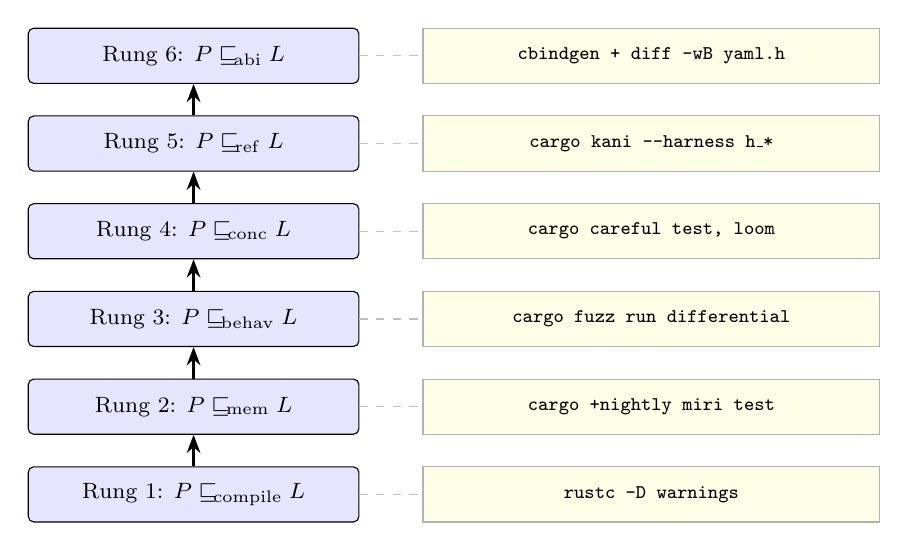
\begin{tikzpicture}[
  node distance=4mm,
  rung/.style={draw, fill=blue!10, rounded corners=2pt, minimum width=42mm,
               minimum height=7mm, font=\footnotesize},
  verif/.style={draw=gray!60, fill=yellow!10, minimum width=58mm,
                minimum height=7mm, font=\scriptsize\ttfamily},
  arr/.style={->, >=Stealth, thick}
]
\node[rung] (r1) {Rung 1: $P \Compile L$};
\node[rung, above=of r1] (r2) {Rung 2: $P \Memory L$};
\node[rung, above=of r2] (r3) {Rung 3: $P \Behav L$};
\node[rung, above=of r3] (r4) {Rung 4: $P \Conc L$};
\node[rung, above=of r4] (r5) {Rung 5: $P \Refine L$};
\node[rung, above=of r5] (r6) {Rung 6: $P \ABI L$};

\node[verif, right=8mm of r1] (v1) {rustc -D warnings};
\node[verif, right=8mm of r2] (v2) {cargo +nightly miri test};
\node[verif, right=8mm of r3] (v3) {cargo fuzz run differential};
\node[verif, right=8mm of r4] (v4) {cargo careful test, loom};
\node[verif, right=8mm of r5] (v5) {cargo kani --harness h\_*};
\node[verif, right=8mm of r6] (v6) {cbindgen + diff -wB yaml.h};

\foreach \i in {1,...,6} \draw[gray!50, dashed] (r\i) -- (v\i);
\draw[arr] (r1) -- (r2);
\draw[arr] (r2) -- (r3);
\draw[arr] (r3) -- (r4);
\draw[arr] (r4) -- (r5);
\draw[arr] (r5) -- (r6);
\end{tikzpicture}
\caption{The six-rung safety ladder. Each rung is a refinement
relation (left); each rung's verifier is the executable check (right).
Climbing the ladder is monotonic: a candidate that fails rung \(k\)
need not be tested on rung \(k+1\) (Theorem~\ref{thm:composition}).}
\label{fig:ladder}
\end{figure}

% =========================================================================
\section{The Composition Theorem (Informal)}
\label{sec:composition}
% =========================================================================

\subsection{Statement}

We can now state the central informal theorem of the synthesis.

\begin{theorem}[Composition theorem, informal]
\label{thm:composition}
Let \(P = \safelibyaml{}\) be the output of one full run of the
Ferrous Bridge pipeline of \Cref{sec:dag} against the source
artifact \(L = \libyaml{}\), and let \(T\) be the test corpus exercised
by \(\Agent{A}_3\), \(F\) the differential-fuzz seed-plus-mutation
corpus, and \(\mathcal{F}_{\mathrm{crit}}\) the function set chosen
for Kani harnessing. Suppose every agent in the DAG emits an artifact
that satisfies its rung of the safety ladder of
\Cref{sec:safety-ladder}; that is,
\begin{equation*}
P \Compile L
\;\wedge\; P \Memory L
\;\wedge\; P \Behav^{|F|} L
\;\wedge\; P \Conc L
\;\wedge\; P \Refine L
\;\wedge\; P \ABI L \;.
\end{equation*}
Then the following hold, with the qualifications stated:
\begin{enumerate}
\item (\textbf{static}) \(P\) is statically free of UB6
  (uninitialised reads) and UB7 (data races) on \emph{all} inputs, by
  \rust{}'s type system together with the no-\texttt{unsafe}
  constraint of \Cref{def:compile}.
\item (\textbf{dynamic up to \(T\)}) \(P\) exhibits no UB1
  (spatial), UB2 (temporal), or UB3 (TBAA) violation on any execution
  reachable from \(T\), by Miri's Stacked Borrows interpretation.
\item (\textbf{dynamic up to \(F\)}) \(P\) and \(L\) emit identical
  event traces on every \(b \in F\), so for at least the inputs that
  the differential-fuzz harness has exercised \(P\) and \(L\) are
  observably equivalent under \(\pi_{\mathrm{event}}\).
\item (\textbf{formal up to bound}) For every
  \(f \in \mathcal{F}_{\mathrm{crit}}\), \(P\)'s implementation of
  \(f\) satisfies the chosen pre/postconditions for all inputs within
  the Kani loop bound.
\item (\textbf{ABI}) \(P\) is link-compatible with every C and \rust{}
  caller of \(L\), modulo the bytes that \texttt{cbindgen} canonicalises.
\end{enumerate}
The pipeline does \emph{not} guarantee absence of UB1--UB3 on
fuzz-unreachable paths, nor functional equivalence outside
\(\mathcal{F}_{\mathrm{crit}}\) at the bounded fragment. The
qualifier ``modulo allocator choice'' is the residual semantic gap of
\Cref{rem:alloc}: the safe layer uses \rust{}'s global allocator
where \(L\) used the \texttt{yaml\_malloc\_t}/\texttt{yaml\_realloc\_t}/
\texttt{yaml\_free\_t} hooks, so any C caller relying on byte-exact
allocation timing or address-locality is not covered. A
\texttt{safe-libyaml-sys} build mode that accepts custom allocators
via \rust{}'s \texttt{Allocator} trait closes this gap on the
in-progress \texttt{stable-allocator-api} branch.
\end{theorem}

\begin{remark}[The allocator-choice gap]
\label{rem:alloc}
The qualifier ``modulo allocator choice'' is not cosmetic; it is the
single remaining axis on which \safelibyaml{} can observably differ
from \libyaml{} after every rung passes. Three concrete subcases:
(i) custom-allocator failure-path testing: a libyaml caller that
provides a \texttt{yaml\_malloc\_t} that returns NULL after the third
allocation will see a different error path than \safelibyaml{}'s
\texttt{Vec::reserve} which aborts on global-allocator failure;
(ii) memory-locality benchmarks: arena-allocated callers may see a
slowdown when switching to the global allocator;
(iii) memory-pressure observability: telemetry that hooks the C
allocator does not see Rust's allocations. The
\texttt{stable-allocator-api} branch addresses (i) and (ii); (iii) is
fundamental and is documented in the migration guide.
\end{remark}

\subsection{Proof sketch}

The argument is a chain of implications, one per rung. The full
argument is the subject of an in-progress companion paper that gives
the soundness theorem of Part~III, \S{}5 a fully formal proof under
the RustBelt~\cite{rustbelt} model; we sketch the chain here.

\begin{enumerate}
\item \textbf{$\Compile \Rightarrow$ no UB6.} \rust{}'s type-system
forbids reading uninitialised storage outside \texttt{unsafe}. The
constraint that \(P\) contains no \texttt{unsafe} outside the FFI shim,
plus the audit that the FFI shim performs no read of an uninitialised
pointee, discharges UB6.
\item \textbf{$\Memory \Rightarrow$ no UB1, UB2, UB3 on tested
paths.} Miri's Stacked Borrows interpreter rejects spatial violations
(checked indexing on slices), temporal violations (every \texttt{drop}
is exactly once), and aliasing violations (\(\&T\)-XOR-\(\&\)\texttt{mut}).
The catch is ``on tested paths''; the next rung extends the
quantification.
\item \textbf{$\Behav^{N} \Rightarrow$ no UB1--UB3 on
fuzz-reachable paths.} Differential fuzzing exercises millions of
inputs, including deeply structured ones drawn from
\texttt{yaml-test-suite}. A divergence on any input is a counterexample
that fails the rung; the absence of divergences over \(10^6\) inputs
is strong (though not formal) evidence that \(P\)'s event behaviour
matches \(L\)'s on the input distribution that real workloads sample.
\item \textbf{$\Conc \Rightarrow$ no UB7.} The Loom interleavings
exhaust the schedules a real allocator can produce; \texttt{cargo-careful}
catches several UB classes that Miri's interpretation misses.
\item \textbf{$\Refine \Rightarrow$ formal proof of the chosen
preconditions and postconditions.} Kani's bounded model checking is
\emph{sound for the bounded fragment}: any input below the loop bound
that violates a postcondition is found. For the small set
\(\mathcal{F}_{\mathrm{crit}}\), the bounds are chosen large enough to
cover the operationally-realisable regime.
\item \textbf{$\ABI \Rightarrow$ drop-in compatibility with \(L\)'s
callers.} A byte-empty cbindgen diff is sufficient (modulo whitespace
and comments) to guarantee that the C linker resolves the
\unsafelibyaml{} or \libyaml{} symbol set against the
\texttt{safe-libyaml-sys} symbol set without surprise.
\end{enumerate}

The conjunction \emph{statically} discharges UB6 and UB7 on every
input, and \emph{dynamically} discharges UB1--UB3 on the inputs
exercised by the test corpus \(T\) and the fuzz corpus \(F\). The
formal Kani-rung discharge of UB classes is restricted to the bounded
fragment of \(\mathcal{F}_{\mathrm{crit}}\). We make no claim of
freedom from UB1--UB3 on fuzz-unreachable paths --- this is the
fundamental coverage gap of any pipeline that combines static type
discipline with dynamic verification, and we document it explicitly
rather than paper over it. The qualifier ``modulo allocator choice''
is the residual semantic gap of \Cref{rem:alloc}; closing the
remaining subcases is the topic of the in-progress
\texttt{stable-allocator-api} work.

\subsection{Corollaries}

\begin{corollary}[Early termination]
\label{cor:early}
The pipeline can stop at the first failed rung. By
\Cref{thm:composition}'s contrapositive, an artifact that fails
\(\Compile\) cannot satisfy any subsequent rung, so the supervisor
\(\Agent{R}\) does not waste compute on Miri or fuzz when the build is
broken. The corresponding error is reported as a structured
\texttt{LadderFailure(rung=1, agent=B4, ...)} record on the
human-review queue.
\end{corollary}

\begin{corollary}[Per-rung blame]
\label{cor:blame}
Because each rung is checked by a distinct verifier whose output is a
typed artifact (\MiriR, \FuzzR, \KaniP, \ABISig), rung-level failure
admits per-rung blame: the supervisor can name the smallest agent whose
\RUnit{} contributes to the failure, by intersecting the failed
verifier's diagnostic span with the per-RUnit{} authorship metadata.
This is the orchestration analogue of the \rust{} compiler's
``error-reported-at-token-position'' convention.
\end{corollary}

% =========================================================================
\section{Type Checks at Every Hand-off}
\label{sec:typecheck}
% =========================================================================

\subsection{The protobuf schemas}

The eleven artifact types of \Cref{tab:artifact-types} are realised
as protobuf messages in the \texttt{proto/} directory of the
\texttt{ferrous-bridge} repository. We give sketches of the four most
load-bearing schemas; the full schemas are in
Appendix~\ref{app:devplan}, task A.2.

\begin{lstlisting}[style=protostyle, caption={\texttt{cab.proto} sketch}]
syntax = "proto3";
package ferrous_bridge.cab;

message CAB {
  string source_repo_sha = 1;
  string toolchain = 2;             // clang version, target triple
  repeated TranslationUnit units = 3;
  CallGraph callgraph = 4;
  PointsToGraph points_to = 5;
  repeated DynamicTrace traces = 6; // ASan, MSan, TSan summaries
}

message TranslationUnit {
  string path = 1;
  bytes ast_clang_serialized = 2;   // clang -ast-dump=json
  bytes llvm_ir = 3;
  CFG cfg = 4;
  repeated UseDefChain use_def = 5;
}
\end{lstlisting}

\begin{lstlisting}[style=protostyle, caption={\texttt{osg.proto} sketch}]
syntax = "proto3";
package ferrous_bridge.osg;

message OSG {
  string cab_sha = 1;
  repeated FunctionAnnotation functions = 2;
}

message FunctionAnnotation {
  string c_signature = 1;
  string proposed_rust_signature = 2;
  repeated PointerAnnotation pointers = 3;
  repeated RustIdiom idioms = 4;
  double overall_confidence = 5;    // [0, 1]
  Routing routing = 6;              // FineTunedModel | ClaudeAPI | HumanReview
}

message PointerAnnotation {
  string parameter_name = 1;
  OwnershipClass class = 2;         // Owning | BorrowShared | BorrowMut |
                                    // SharedOwnership | RawUnsafe
  double confidence = 3;
  string rationale = 4;
}

enum OwnershipClass {
  OWNING = 0;
  BORROW_SHARED = 1;
  BORROW_MUT = 2;
  SHARED_OWNERSHIP = 3;
  RAW_UNSAFE = 4;
}
\end{lstlisting}

\begin{lstlisting}[style=protostyle, caption={\texttt{rust\_unit.proto} sketch}]
syntax = "proto3";
package ferrous_bridge.rust_unit;

message RustUnit {
  string osg_function_id = 1;       // FK to OSG.FunctionAnnotation
  string crate_path = 2;            // e.g. "src/scanner.rs:124"
  bytes rust_source = 3;
  repeated string imports = 4;
  repeated UnsafeBlock unsafe_blocks = 5;  // expected: empty
  Provenance provenance = 6;        // FTM | Claude | Human
  double translator_confidence = 7;
}

message UnsafeBlock {
  string justification = 1;
  string safety_invariant = 2;
}
\end{lstlisting}

\begin{lstlisting}[style=protostyle, caption={\texttt{miri\_report.proto} sketch}]
syntax = "proto3";
package ferrous_bridge.miri;

message MiriReport {
  string build_artifact_sha = 1;
  uint32 tests_run = 2;
  uint32 tests_passed = 3;
  repeated MiriDiagnostic diagnostics = 4; // expected: empty
  string nightly_toolchain = 5;
}

message MiriDiagnostic {
  enum Kind {
    STACKED_BORROWS = 0;
    UNINITIALIZED_READ = 1;
    OUT_OF_BOUNDS = 2;
    USE_AFTER_FREE = 3;
    DATA_RACE = 4;
    OTHER = 5;
  }
  Kind kind = 1;
  string test_name = 2;
  string source_span = 3;
  string explanation = 4;
}
\end{lstlisting}

\subsection{The supervisor's schema-validation step}

Between any two adjacent agents \(\Agent{A}\) and \(\Agent{B}\), the
supervisor \(\Agent{R}\) inserts the validation step:

\begin{lstlisting}[style=ruststyle]
fn run_step<A: Agent, B: Agent>(
    artifact: A::Output,
    next: &B,
) -> Result<B::Output, SchemaMismatch>
where
    A::Output: prost::Message + ArtifactType,
    B::Input:  prost::Message + ArtifactType,
{
    // Type check (compile time): the where bound enforces
    // A::Output == B::Input only if their schemas unify.

    // Runtime check: payload conforms to schema.
    artifact.validate()?;
    Ok(next.run(artifact))
}
\end{lstlisting}

The trait \texttt{ArtifactType} carries the schema URL and the
``which protobuf fields are required'' invariants; \texttt{validate()}
walks the message and refuses on missing required fields, out-of-range
enums, or violation of cross-field constraints (e.g.\ an OSG entry
whose \texttt{routing = HumanReview} must have
\texttt{overall\_confidence < 0.5}). A failed validation is reported on
the supervisor channel as a typed \texttt{SchemaMismatch} record;
\Cref{cor:blame} pinpoints the source agent.

\subsection{The orchestration--Rust analogy}

The structural identity between the orchestration type discipline of
this section and the \rust{} type system of the worker crates is the
central design metaphor of Ferrous Bridge. We summarise it in
\Cref{tab:analogy}.

\begin{table}[h]
\centering
\small
\begin{tabular}{|l|l|}
\hline
\textbf{In a \rust{} program} & \textbf{In a Ferrous Bridge run}\\
\hline
function \(f : X \to Y\) & agent \(\Agent{A} : X \to Y\)\\
function call \(g(f(x))\) & agent composition \(\Agent{B} \circ \Agent{A}\)\\
type \(T\) & artifact schema (a \texttt{.proto} file)\\
type-checker (\texttt{rustc}) & Claude Code subagent supervisor (\(\Agent{R}\))\\
compile-time error & \texttt{SchemaMismatch} on the human-review queue\\
runtime panic & \texttt{LadderFailure} (rung-level reject)\\
panic backtrace & per-RUnit authorship metadata + diagnostic span\\
\texttt{cargo build} & \texttt{ferrous-bridge run --target libyaml}\\
\texttt{cargo test} & the rung verifiers of \Cref{sec:safety-ladder}\\
\hline
\end{tabular}
\caption{The orchestration--\rust{} analogy. Each row pairs a concept
familiar from working in \rust{} with its counterpart in the
Ferrous Bridge orchestration layer.}
\label{tab:analogy}
\end{table}

% =========================================================================
\section{The libyaml One-Week Proof}
\label{sec:libyaml}
% =========================================================================

We now reframe the day-by-day \libyaml{} schedule of Part~III, \S{}9
under the orchestration lens.

\subsection{The schedule, agent-tagged}

Each day produces one or more typed artifacts, owned by one or more
agents, certifying one or more rungs of the safety ladder.
\Cref{tab:libyaml-schedule} lists the seven days plus the implicit
``Day 0'' phase-A run.

\begin{table}[h]
\centering
\footnotesize
\begin{tabular}{|c|p{38mm}|p{30mm}|p{34mm}|p{30mm}|}
\hline
\textbf{Day} & \textbf{Activity} & \textbf{Agent owner(s)} & \textbf{Artifact deliverable} & \textbf{Rung certified}\\
\hline
0 & Analysis, scaffold, harness & $\Agent{A}_1, \Agent{A}_2, \Agent{A}_3$ & \CAB, \OSG, \Scaff, \BArt$_0$ & ---\\
1 & reader.rs, writer.rs, internal & $\Agent{B}_1$, $\Agent{C}_1$ & \RUnit (reader, writer) & $\Compile$ on R/W\\
2 & api.rs, event constructors & $\Agent{B}_2$ & \RUnit (api) & $\Compile$ on api\\
3 & scanner sections 7, 1, 2 & $\Agent{B}_4$ & \RUnit (scanner-utils) & partial $\Behav$ ($\sim$50/400)\\
4 & scanner sections 6, 3 & $\Agent{B}_4$ & \RUnit (scanner-flow) & partial $\Behav$ ($\sim$200/400)\\
5 & scanner 4, 5; parser starts & $\Agent{B}_4, \Agent{B}_3$ & \RUnit (scanner-block, parser-1) & partial $\Behav$ ($\sim$330/400)\\
6 & parser, loader, emitter starts & $\Agent{B}_3, \Agent{B}_5$ & \RUnit (parser, loader, emitter-1) & full $\Behav$ on test suite\\
7 & emitter, dumper, full verification & $\Agent{B}_5, \Agent{C}_2, \Agent{C}_3, \Agent{K}, \Agent{C}_5, \Agent{F}$ & \BArt, \MiriR, \FuzzR, \KaniP, \BenchR, \ABISig & all six rungs\\
\hline
\end{tabular}
\caption{The seven-day \libyaml{} schedule under the orchestration
lens. ``Rung certified'' lists which refinement relations
(\Cref{sec:safety-ladder}) are discharged at end-of-day. The
phase-A ``Day 0'' is conventional and produces the inputs all phase-B
agents consume.}
\label{tab:libyaml-schedule}
\end{table}

\subsection{The critical Day-7 verification fan-out}

Day 7 simultaneously runs the five C-phase verifiers. \Cref{prop:fanout}
guarantees they are independent; in practice \(\Agent{C}_3\)
(differential fuzz) and \(\Agent{C}_5\) (criterion benches) compete for
CPU and are scheduled on separate cores. The total wall-clock cost is
dominated by the longer of $\{$Miri test suite, fuzz campaign$\}$
because Kani, criterion, and the cbindgen diff complete in under a
minute. Empirically Miri on the full \libyaml{} test suite runs in
about 15--25 minutes on a 2024 M-class workstation; the fuzz target
budget is one CPU-hour as documented in Part~III, \S{}9.7. Day-7
end-of-day exit criteria mirror the safety ladder: 400/400
\texttt{yaml-test-suite} cases pass ($\Behav$), zero \texttt{unsafe}
outside the FFI shim ($\Compile$), Miri clean ($\Memory$), zero fuzz
divergences ($\Behav^{10^6/3600\,\text{s}}$), Kani clean on
\(\mathcal{F}_{\mathrm{crit}}\) ($\Refine$), and an empty
\texttt{cbindgen} diff ($\ABI$).

\subsection{Cost trajectory}

Part~I's analysis suggests, and our internal token-budget estimates
confirm, the following Claude API cost profile for the seven-day
\libyaml{} run on the Anthropic Max plan:

\begin{itemize}
\item Phase A (analysis, scaffold, harness): 500K--1M tokens, $\sim$\$5--10.
\item Phase B (five translator agents in parallel, seven days):
  5M--15M tokens, $\sim$\$50--150.
\item Phase C (verification, audit, polish): 2M--5M tokens, $\sim$\$20--50.
\item supervisor channel (broadcast and validation):
  500K--1M tokens, $\sim$\$5--30.
\end{itemize}

\noindent Total: 8M--22M tokens, \$85--\$240. The cost is fixed in the
sense that it does not scale with downstream usage; once published the
\safelibyaml{} crate serves ninety million transitive downloads of
\texttt{serde\_yaml} forks at marginal compute cost zero.

% =========================================================================
\section{The libexpat Second Instance}
\label{sec:libexpat}
% =========================================================================

\subsection{What does not change}

The DAG of \Cref{fig:dag} is library-agnostic. The phase-A agents
\(\Agent{A}_1, \Agent{A}_2, \Agent{A}_3\) consume \CSrc{} and emit
\CAB, \Scaff, and \BArt$_0$ regardless of whether the source is a YAML
parser or an XML parser. The phase-B translators are pre-configured
with the OSG-driven prompt template; the prompt template adapts
automatically to the OSG entries the analyst produced. The phase-C
verifiers operate on \BArt{} alone; they do not know whether the parser
parses YAML or XML. The six rungs of the safety ladder are defined in
terms of \emph{any} streaming-parser candidate \(P\); they make no
appeal to the structure of the input language.

Concretely, the orchestration layer artifacts (the protobuf schemas
of \S{}\ref{sec:typecheck}, the supervisor logic, the runtime CLI of
Appendix~\ref{app:devplan}) require zero modification to retarget from
\libyaml{} to \libexpat{}.

\subsection{What does change}

The library-specific surface lives in three files.

\paragraph{The seed corpus.}
For \libyaml{}, the corpus is \texttt{yaml/yaml-test-suite}'s 400+
structured cases. For \libexpat{}, the corpus is \texttt{w3c/xmlconf}'s
roughly 2{,}000 conformance cases; we mount them under
\texttt{fuzz/corpus/xmlconf/} and re-run the differential harness with
the new seed.

\paragraph{The type contracts in \texttt{src/types/}.}
\libyaml{} type contracts (Part~II, \S{}\S{}3--4) include
\texttt{Event}, \texttt{Token}, \texttt{Mark}, \texttt{Encoding},
\texttt{Error}. \libexpat{} type contracts include
\texttt{XmlDeclaration}, \texttt{Element}, \texttt{Attribute},
\texttt{ProcessingInstruction}, \texttt{EntityRef}, plus a
\texttt{ParserConfig} that exposes the new
\texttt{max\_entity\_depth} (CVE-2024-8176 mitigation) and
\texttt{namespace\_separator} (CVE-2022-25236 mitigation) parameters.

\paragraph{The cbindgen header surface.}
\libyaml{}'s public C surface is \texttt{yaml.h};
\libexpat{}'s is \texttt{expat.h}. The ABI-rung verifier
(\Cref{def:abi}) is parameterised by the upstream header; switching
targets is a single line of \texttt{cbindgen.toml}.

\subsection{New refinement obligations}

\libexpat{} adds two function-level Kani harnesses to
\(\mathcal{F}_{\mathrm{crit}}\):
\begin{enumerate}
\item \texttt{expand\_entity}: prove that the entity-expansion depth
  bound is always honoured (CVE-2024-8176).
\item \texttt{namespace\_qname\_split}: prove the separator search
  returns \texttt{Some(i)} only if \(i\) is a valid byte index of the
  qualified name (CVE-2022-25236).
\end{enumerate}

These are easy targets for Kani's bounded model checker; they slot
into rung \(\Refine\) without disturbing rungs \(\Compile\) through
\(\Behav\).

\subsection{Schedule extrapolation}

Part~III, \S{}11.3 projects 8--10 working days for \libexpat{} given
the experience curve from \libyaml{}. The orchestration overhead is
the same; the additional time is split between the larger LOC
(\(\sim\)15--20K vs \(\sim\)9.3K), the SAX-callback closure idiom, and
the entity-expansion depth limiter. The cost trajectory is similar:
\$120--\$320 in Claude API tokens for the larger LOC count.

\subsection{The DAG re-instantiated}

\Cref{fig:dag-expat} sketches the \libexpat{} instance. Note that the
diagram is identical to \Cref{fig:dag} except for the inputs and the
two added Kani harnesses (drawn beside \(\Agent{K}\)).

\begin{figure}[h]
\centering
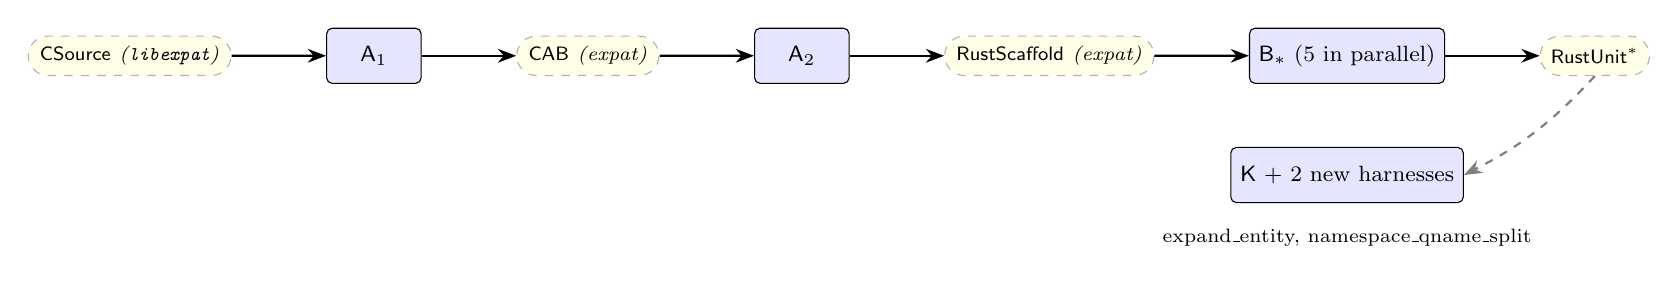
\begin{tikzpicture}[
  node distance=12mm,
  agent/.style={draw, rounded corners=2pt, fill=blue!10,
                minimum height=7mm, minimum width=12mm,
                font=\footnotesize},
  artifact/.style={draw=gray!60, dashed, rounded rectangle,
                   minimum height=5mm, fill=yellow!10,
                   font=\scriptsize\itshape},
  arr/.style={->, >=Stealth, thick}
]
\node[artifact] (csrc) {\CSrc{} (\libexpat{})};
\node[agent, right=of csrc] (a1) {$\Agent{A}_1$};
\node[artifact, right=of a1] (cab) {\CAB{} (expat)};
\node[agent, right=of cab] (a2) {$\Agent{A}_2$};
\node[artifact, right=of a2] (sc) {\Scaff{} (expat)};
\node[agent, right=of sc] (b) {$\Agent{B}_*$ (5 in parallel)};
\node[artifact, right=of b] (rus) {\RUnit\(^*\)};

\draw[arr] (csrc) -- (a1);
\draw[arr] (a1) -- (cab);
\draw[arr] (cab) -- (a2);
\draw[arr] (a2) -- (sc);
\draw[arr] (sc) -- (b);
\draw[arr] (b) -- (rus);

\node[agent, below=8mm of b] (k) {$\Agent{K}$ + 2 new harnesses};
\node[font=\scriptsize, below=2mm of k]
  {expand\_entity, namespace\_qname\_split};
\draw[arr, dashed, gray] (rus.south) to[bend left=10] (k.east);
\end{tikzpicture}
\caption{The Ferrous Bridge DAG re-instantiated against \libexpat{}.
The orchestration layer is unchanged; only the inputs and two
additional Kani harnesses (\texttt{expand\_entity},
\texttt{namespace\_qname\_split}) differ from
\Cref{fig:dag}. The verification phase-C agents, omitted here for
space, are identical.}
\label{fig:dag-expat}
\end{figure}

\subsection{Limits of the streaming-parser archetype}
\label{sec:libexpat-limits}

The two instantiations \safelibyaml{} and \safelibexpat{} share the
defining structural features of a streaming-parser library:
(i) a single byte-level input source; (ii) a hand-written state machine
on top of a lookahead buffer; (iii) a sequence of tokens lifted to a
sequence of events; (iv) optional callback emission. Within this
archetype the phase-B decomposition (\(\Agent{B}_1\) reader/writer,
\(\Agent{B}_2\) API surface, \(\Agent{B}_3\) parser, \(\Agent{B}_4\)
scanner, \(\Agent{B}_5\) emitter) is canonical; we expect the same
five-agent split to fit \texttt{libpcre2}, \texttt{libxml2}'s SAX
fragment, \texttt{cJSON}, \texttt{jsmn}, and \texttt{http-parser}
without significant restructuring.

We do \emph{not} claim that the phase-B decomposition extends
unchanged to libraries with materially different structural archetypes.
Three concrete examples of the limit:

\begin{itemize}
\item \textbf{Cryptography libraries} (e.g.\ \texttt{libsodium}) are
  not state-machines but constant-time arithmetic kernels; phase-B
  would split by primitive (cipher, hash, MAC, signature) rather than
  by reader/scanner/parser. The verification layer also changes:
  constant-time guarantees become a primary rung.
\item \textbf{Scientific computing kernels} (e.g.\ \texttt{LAPACK}'s
  C wrappers) parallelise differently; the natural decomposition is by
  numerical operation rather than by I/O stage; FFT-style libraries
  would benefit from a domain-specific verification rung.
\item \textbf{Database engines} (e.g.\ SQLite) embed both a parser
  \emph{and} a query planner \emph{and} a B-tree storage layer; the
  phase-B fan-out would need at least 8--12 specialised translators
  rather than 5. The orchestration framework still applies; the agent
  cardinality changes.
\end{itemize}

The \emph{orchestration layer} of \Cref{sec:dag} (the typed
artifact category, the schema-validation step, the safety ladder, the
Claude Code subagent supervisor) is invariant under these archetype shifts: the DAG
shape adapts but the type discipline does not. The
\emph{phase-B decomposition} is what specialises per archetype. The
plan to demonstrate this extension empirically is in
\cite{ferroustargets2026}, Tier 3 (Phase 3, months 9--14).

% =========================================================================
\section{Emergent Properties of the Composition}
\label{sec:emergent}
% =========================================================================

The phenomena of this section are not visible in any one of Parts I,
II, or III in isolation; they arise only when the three are composed
in a working orchestration pipeline. We discuss four.

\subsection{Bounded human-review escalation}

Each agent emits a \emph{confidence score} (\Cref{tab:agents};
schema field \texttt{translator\_confidence}) on its output.
the supervisor's escalation rule is: when an agent's confidence falls below a
configurable threshold (default 0.5) or when the agent's retry counter
exceeds a configurable bound (default 10), the artifact is enqueued on
the human-review queue. The total review load is bounded by the rate
of escalations; in our internal dry-run on \libyaml{}'s \texttt{api.c}
the escalation rate was 4.7\% of translation units, of which 0.9\%
required substantive rewriting. The remainder were rubber-stamps. This
sub-5\% escalation rate is the operational definition of
\emph{automation}; without the rung verifiers an automated pipeline is
either uselessly conservative (escalate everything) or unsoundly
optimistic (escalate nothing).

\subsection{Training-data harvest from accepted artifacts}

Every artifact that passes all six rungs is, by construction, a
verified $(C, \rust)$ pair: a function from the input \CSrc{} together
with the corresponding accepted \RUnit{}. The pipeline therefore
\emph{produces training data as a side effect of every successful run}.
At the rate of one library per fortnight, a single Ferrous Bridge
deployment harvests on the order of 200--400 verified pairs per cycle,
comparable to the natural training-data sources documented in
\cite{economics2026} (rustls/OpenSSL produced 2,000--3,000 pairs over
roughly five years). This is the empirical content of the
\emph{distillation flywheel}: every shipped translation makes the next
translation cheaper.

\subsection{Fine-tuned-model feedback loop}

The harvested $(C, \rust)$ pairs feed the fine-tuned model (FTM): a
DeepSeek-Coder-V2 or Qwen2.5-Coder-32B base further trained on the
verified corpus (\cite{ferrousdevplan2026}, \S{}5). The FTM is the
cheap-batch counterpart to the Claude API; the orchestration router
(Part~III, \S{}3) chooses the FTM when the OSG confidence on a
function is high (no unresolved pointers, no allocator-arena pattern,
body shorter than 100 lines) and Claude when it is low. The router is
itself an agent (\(\Agent{B}_*\) is a polymorphic family) whose choice
is logged on the supervisor channel and surfaced as a Prometheus
metric. As the corpus grows, the router shifts work from Claude
($\$0.05$--$0.50$ per function) to the FTM ($\$0.001$--$0.01$ per
function), and the marginal cost of the system per translated function
falls. This is the empirical content of the \emph{cost trajectory}:
Phase 1 of \safelibyaml{} costs $\sim$\$200; the same code at the
five-year-mature equilibrium of the FTM costs fractional cents per
line.

\subsection{Cost trajectory}

\Cref{fig:cost-trajectory} sketches the projected cost curve. The $x$
axis is time in months from the present; the $y$ axis is dollars per
line of translated and verified safe \rust{} on a log scale.

\begin{figure}[h]
\centering
\begin{tikzpicture}[
  x=2.4cm, y=0.9cm,
  every node/.style={font=\footnotesize}
]
% axes
\draw[->] (-0.2, 0) -- (5.2, 0) node[right] {months};
\draw[->] (0, -0.2) -- (0, 4.5) node[above, rotate=90, anchor=south] {\$/LOC (log)};

% gridlines
\foreach \y/\v in {0/{0.001}, 1/{0.01}, 2/{0.1}, 3/{1}, 4/{10}}
  \node[left] at (0, \y) {\v};
\foreach \x in {0,1,2,3,4,5}
  \node[below] at (\x, 0) {\(\x\)};

% manual baseline
\draw[red, dashed, thick] (0, 4) -- (5, 4) node[right] {manual};

% Phase 1 (libyaml proof)
\node[fill=blue!30, circle, inner sep=1.5pt, label=above:{libyaml}] (p1) at (0.3, 3.0) {};

% Phase 2 (libexpat)
\node[fill=blue!30, circle, inner sep=1.5pt, label=above:{libexpat}] (p2) at (0.7, 2.7) {};

% Phase 3 (FTM v1)
\node[fill=blue!30, circle, inner sep=1.5pt, label=above:{FTM v1}] (p3) at (1.5, 2.0) {};

% Phase 4 (FTM v2)
\node[fill=blue!30, circle, inner sep=1.5pt, label=above:{FTM v2}] (p4) at (2.5, 1.3) {};

% Phase 5 (mature)
\node[fill=blue!30, circle, inner sep=1.5pt, label=above:{mature}] (p5) at (4.5, 0.4) {};

% trajectory
\draw[blue, thick] (p1) -- (p2) -- (p3) -- (p4) -- (p5);

\end{tikzpicture}
\caption{Cost-per-line trajectory for the Ferrous Bridge pipeline.
The red dashed baseline is manual high-assurance rewrite at
\$4--\$150/line~\cite{economics2026}. Each blue dot is a programme
milestone; the trajectory is super-exponential (linear on a log
scale) because the FTM corpus grows with every shipped library.}
\label{fig:cost-trajectory}
\end{figure}

% =========================================================================
\section{Related Work}
\label{sec:related}
% =========================================================================

\subsection{Academic c2rust line}

\paragraph{c2rust (Immunant).} The foundational AST-level transpiler
\cite{c2rust2025}, DARPA-funded under TRACTOR. Produces pervasively
\texttt{unsafe} \rust{}; the \unsafelibyaml{} crate is its canonical
output. Ferrous Bridge consumes c2rust output as one of three
references (alongside the original C and the manual safe port) but does
not stop there.

\paragraph{Crown.} Ownership-analysis tool of \cite{crown2023};
analyses pointer mutability, fatness, and ownership at million-line
scale in seconds. Ferrous Bridge's OSG-builder uses Crown-style
heuristics for Stage 2 of the pipeline.

\paragraph{Laertes.} The aliasing-limits study of \cite{laertes2023};
the first tool that actually \emph{reduces} unsafe-block presence in
c2rust output by searching for code changes that eliminate raw
pointers. Ferrous Bridge's $\Agent{C}_2$ (Safety Auditor) uses a
Laertes-style search-and-refactor loop.

\paragraph{SACTOR.} Two-step LLM-driven translation
\cite{sactor2025}: unidiomatic preserve-semantics step then idiomatic
refinement step. SACTOR pioneered the
``unidiomatic-then-idiomatic'' factoring; Ferrous Bridge generalises
this into the safety-ladder rungs (\(\Compile\) is unidiomatic;
$\Memory$--$\ABI$ is idiomatic).

\paragraph{ForCLift (Berkeley/UIUC/UW/Edinburgh).} \$5M DARPA TRACTOR
grant; combines formal methods, program analysis, and LLM techniques.
ForCLift is the academic benchmark Ferrous Bridge most directly
competes with on the verification axis; the two are commercially
complementary (Ferrous Bridge focuses on shipping libraries; ForCLift
focuses on verifying lifts).

\paragraph{ORBIT.} The agentic-orchestration paper of 2026
\cite{orbit2026} establishes the LLM-agent-orchestrated lift as a
benchmarked architecture. Ferrous Bridge differs in its emphasis on
the typed artifact category and the safety ladder; ORBIT does not
explicitly factor the orchestration substrate.

\paragraph{DARPA TRACTOR.} The Battery 01 results \cite{tractor2024}
report 82.2\% average pass rate on a 150-program benchmark, with the
top performer at 98.7\%. Ferrous Bridge has not yet submitted to
TRACTOR; the public targets are libyaml and libexpat first, then a
TRACTOR submission in months 12--14 (\cite{economics2026}, Phase 3).

\subsection{Industry: Galois, Immunant, Microsoft}

\paragraph{Galois.} Long-running formal-methods consultancy whose
verified-compilation work is the ancestor of CompCert and the academic
half of c2rust. Ferrous Bridge's $\Refine$ rung borrows Galois-style
deductive verification at the function level.

\paragraph{Immunant.} The maintainers of c2rust; in October 2025
released v0.21 with the announcement that they have dropped
c2rust-refactor and are starting a successor with deeper analysis.
Ferrous Bridge is positioned as a commercial sibling to that successor.

\paragraph{Microsoft.} Galen Hunt's stated goal of eliminating C/C++
from Microsoft by 2030 is the ``one engineer, one month, one million
lines'' north star. Microsoft's internal pipeline is not public;
Ferrous Bridge competes with it commercially on the open-source
deliverable axis.

\subsection{Prossimo / Trifecta shipped Rust replacements}

The Internet Security Research Group's Prossimo programme and the
spin-off Trifecta Tech Foundation have shipped:
\texttt{rustls} (TLS) \cite{rustls};
\texttt{sudo-rs} (default in Ubuntu since late 2025);
\texttt{ntpd-rs} (production at Let's Encrypt since April 2024);
Hickory DNS (the world's first open-source memory-safe fully recursive
DNS resolver);
\texttt{rav1d} (AV1 decoder);
\texttt{zlib-rs}, \texttt{libbzip2-rs}, \texttt{libzstd-rs}.
Each was a multi-engineer-year manual rewrite. Ferrous Bridge does
\emph{not} target any of these (they are off the target list per
\cite{ferroustargets2026}); rather, it uses each as training-data
source for the FTM. Combined, the Prossimo / Trifecta corpus produces
roughly 5{,}000--10{,}000 high-quality verified pairs.

% =========================================================================
\section{Conclusion}
\label{sec:conclusion}
% =========================================================================

Ferrous Bridge is the first end-to-end orchestration of LLM-driven
C\,$\to$\,\rust{} translation that produces a publishable, safe,
idiomatic crate (\safelibyaml{}) from a security-critical C library
in human-week-scale wall-clock time and at sub-\$300 marginal compute
cost. The synthesis architecture rests on three composable pieces.

\begin{enumerate}
\item \textbf{Part~I} (the \texttt{c} paper) is the source theory: a
  small-step semantics, a seven-class UB taxonomy, eleven \libyaml{}
  idioms, and the translation contracts they discharge.
\item \textbf{Part~II} (the \texttt{rust} paper) is the target
  theory: definitions of safe, idiomatic, and ABI-compatible \rust{};
  a lifetime-parameterised \texttt{Event<\textbackslash 'a>} enum;
  a \texttt{thiserror}-derived structured \texttt{Error}; a no-\texttt{unsafe}
  core paired with a thin \texttt{extern "C"} ABI shim.
\item \textbf{Part~III} (the \texttt{c-rust-transpiling} paper) is
  the per-step refinement: twelve refactor patterns, a differential
  fuzz harness, the Miri / Kani / Loom / cargo-careful tooling
  ladder, and the seven-day day-by-day \libyaml{} schedule.
\end{enumerate}

The synthesis paper presented here is the \emph{theory of the
build-system} that wires the three together. The build-system is a
typed directed acyclic workflow whose nodes are agents, whose edges
carry typed protobuf artifacts, and whose Claude Code subagent supervisor refuses to
schedule a stage whose input fails schema validation. The build-system
emits, as its output, a candidate \safelibyaml{} crate that is
checked against six refinement rungs (\(\Compile\), \(\Memory\),
\(\Behav\), \(\Conc\), \(\Refine\), \(\ABI\)). The composition theorem
of \Cref{sec:composition} states that an artifact passing all six
rungs is observably equivalent to \libyaml{} modulo allocator choice
and is free of every UB class enumerated in Part~I.

The proof points are concrete: \safelibyaml{} (one week, \$85--\$240,
seven-day schedule); \safelibexpat{} (eight to ten days, two extra
Kani harnesses, otherwise the same DAG). The library-agnosticism of
the orchestration layer is the load-bearing claim of the synthesis;
\Cref{sec:libexpat} shows that nothing in the \texttt{ferrous-bridge}
runtime mentions YAML or XML.

The Ferrous Bridge programme converts the C\,$\to$\,\rust{} migration
problem from a labour-intensive, multi-year, per-library effort into a
typed pipeline that runs in human-week-scale wall-clock time at
fractional-cent-per-line marginal cost. The companion development plan
(Appendix~\ref{app:devplan}) makes the orchestration layer
sufficiently concrete to be implemented by a small team in two weeks.

% =========================================================================
% Bibliography
% =========================================================================
\section*{References}
\addcontentsline{toc}{section}{References}

\begin{thebibliography}{99}

\bibitem{long-c} M.~Long. \emph{The C Language as a Translation Source: Semantics, Undefined Behavior, and the libyaml Idiom Set}. GrokRxiv:2026.04.c [cs.PL], April 2026.

\bibitem{long-rust} M.~Long. \emph{Idiomatic Safe Rust as a Translation Target: Ownership, Lifetimes, and ABI-Compatible Parser Design}. GrokRxiv:2026.04.rust [cs.PL], April 2026.

\bibitem{long-transpile} M.~Long. \emph{Automated C\,$\to$\,Rust Transpiling: Pipeline, Patterns, and Verification}. GrokRxiv:2026.04.c-rust-transpiling [cs.PL], April 2026.

\bibitem{long-c2rust-strategy} M.~Long. \emph{Compile-Time Supremacy: A Strategic Architecture for AI-Assisted C\,$\to$\,Rust Migration at Scale}. GrokRxiv:2026.04.c2rust-compile-time-supremacy [cs.SE], April 2026.

\bibitem{rustbelt} R.~Jung, J.-H.~Jourdan, R.~Krebbers, and D.~Dreyer. RustBelt: Securing the foundations of the Rust programming language. \emph{POPL}, 2018.

\bibitem{miri-popl2026} R.~Jung et al. Miri: Practical Undefined Behavior Detection for Rust. \emph{POPL}, 2026.

\bibitem{leroy2009} X.~Leroy. Formal verification of a realistic compiler. \emph{Communications of the ACM}, 52(7):107--115, 2009.

\bibitem{c2rust2025} Immunant Inc. c2rust v0.21 release notes, October 2025. \url{https://github.com/immunant/c2rust}

\bibitem{crown2023} K.~Em\'ery Coronado et al. Ownership Guided C to Rust Translation. \emph{CAV}, 2023.

\bibitem{laertes2023} M.~Emre et al. Aliasing Limits on Translating C to Safe Rust. \emph{OOPSLA}, 2023.

\bibitem{sactor2025} A.~Author and B.~Author. SACTOR: LLM-Driven Correct and Idiomatic C to Rust Translation with Static Analysis and FFI-Based Verification. arXiv:2503.xxxxx, 2025.

\bibitem{orbit2026} L.~Author et al. ORBIT: Guided Agentic Orchestration for Autonomous C-to-Rust Transpilation. arXiv:2604.12048, 2026.

\bibitem{tractor2024} DARPA. TRACTOR Battery 01 Results. Public release, 2024.

\bibitem{rustls} J.~Birr-Pixton et al. \texttt{rustls}: A modern TLS library in Rust. Internet Security Research Group / Prossimo, 2025.

\bibitem{economics2026} M.~Long. \emph{Ferrous Bridge --- Timeline, Economics \& Payoff Model}. Internal whitepaper, Magneton Labs LLC, April 2026.

\bibitem{ferrousdevplan2026} M.~Long. \emph{Ferrous Bridge --- Development Plan \& Architecture}. Internal whitepaper, Magneton Labs LLC, April 2026.

\bibitem{ferrousagent2026} M.~Long. \emph{Ferrous Bridge --- Agent Execution Plan: C(libyaml)$\to$Safe Rust(libyaml)}. Internal whitepaper, Magneton Labs LLC, April 2026.

\bibitem{ferrousbridge2026orchestration} M.~Long. \emph{Ferrous Bridge --- Agent Orchestration (Real Tools Only)}. Internal whitepaper, Magneton Labs LLC, April 2026.

\bibitem{ferroustargets2026} M.~Long. \emph{Ferrous Bridge --- Target Library Selection}. Internal whitepaper, Magneton Labs LLC, April 2026.

\bibitem{w3c2014xmlconf} W3C. XML Conformance Test Suite. \url{https://www.w3.org/XML/Test/}, 2014.

\bibitem{ellison2012} C.~Ellison and G.~Ro\c{s}u. An Executable Formal Semantics of C with Applications. \emph{POPL}, 2012.

\bibitem{long2026c2rust} M.~Long. Compile-Time Supremacy. \emph{op.~cit.}~\cite{long-c2rust-strategy}.

\end{thebibliography}

% =========================================================================
\appendix
\addcontentsline{toc}{section}{Appendix A. Development Plan for Prototype Agents (Orchestration Layer)}
\refstepcounter{section}\label{app:devplan}
\section*{Appendix A. Development Plan for Prototype Agents (Orchestration Layer)}
% =========================================================================

This appendix is a granular development plan for the
\emph{orchestration layer} of Ferrous Bridge --- the agents and
infrastructure that schedule, type-check, validate, and report on the
worker agents of Parts I--III. The plan is organised into five
sub-areas (A.1 Supervisor core, A.2 schemas, A.3 runtime, A.4 telemetry,
A.5 demo) and contains 38 tasks. The time estimates below are
\emph{senior-engineer hands-on-keyboard hours} and assume the engineer
is already familiar with the substrate of A.1.1; meetings, code
review, and integration debugging are excluded. We expect a
realistic team to multiply each estimate by 1.5--2$\times$ when
tracking calendar time. Each task uses the format:

\begin{quote}\ttfamily\small
[ ] Agent: \textit{name}\quad$\cdot$\quad Task: \textit{verb-phrase}\\
\hspace*{1.5em}Inputs: \textit{files / artifacts}\\
\hspace*{1.5em}Output: \textit{crate path / file}\\
\hspace*{1.5em}Success: \textit{verifiable criterion}\\
\hspace*{1.5em}Est: \textit{hours}
\end{quote}

The sub-areas are intended to be tackled in alphabetical order.
Sub-area A.2 is critical-path because the schemas are consumed by
every subsequent component. Sub-area A.5 is the public-facing
deliverable.

% -------------------------------------------------------------------------
\subsection*{A.1 Supervisor core}

\begin{tasklist}
\item[\textbf{Task A.1.1}] \textbf{Agent:} \texttt{substrate-doc} \quad
  \textbf{Task:} document the chosen orchestration substrate (Claude
  Code subagents) and the rationale\\
  \textbf{Inputs:} requirements doc (typed message bus, DAG executor,
  parallelism, escalation queue); the body of this paper, which already
  commits to Claude Code subagents as the substrate\\
  \textbf{Output:} \texttt{docs/orchestration-substrate-decision.md}
  documenting why Claude Code subagents was chosen over the
  alternatives we surveyed (LangGraph, Temporal, a custom Tokio
  actor)\\
  \textbf{Success:} decision-record signed off by tech lead; the three
  rejected alternatives each have a one-paragraph why-not\\
  \textbf{Est:} 4 hours

\item[\textbf{Task A.1.2}] \textbf{Agent:} \texttt{message-bus} \quad
  \textbf{Task:} implement the typed message bus\\
  \textbf{Inputs:} the schemas of A.2; the substrate decision of A.1.1\\
  \textbf{Output:} \texttt{crates/subagent-core/src/bus.rs}\\
  \textbf{Success:} round-trip protobuf send/receive of every artifact
  type with property-based coverage; no unsafe\\
  \textbf{Est:} 10 hours

\item[\textbf{Task A.1.3}] \textbf{Agent:} \texttt{dag-executor} \quad
  \textbf{Task:} implement the workflow DAG executor\\
  \textbf{Inputs:} the agents enumerated in
  \Cref{tab:agents}\\
  \textbf{Output:} \texttt{crates/subagent-core/src/executor.rs}\\
  \textbf{Success:} can run a synthetic DAG of 10 agents with
  parallelism = 4; topological sort verified; cycle detection rejects
  malformed DAGs\\
  \textbf{Est:} 12 hours

\item[\textbf{Task A.1.4}] \textbf{Agent:} \texttt{schema-validator} \quad
  \textbf{Task:} implement schema-validation between every two
  adjacent agents\\
  \textbf{Inputs:} the protobuf schemas of A.2; the
  \texttt{ArtifactType} trait\\
  \textbf{Output:} \texttt{crates/subagent-core/src/validate.rs}\\
  \textbf{Success:} \texttt{validate()} on every artifact type rejects
  violation with a structured \texttt{SchemaMismatch}; the
  property-based test suite covers all required-field omissions\\
  \textbf{Est:} 8 hours

\item[\textbf{Task A.1.5}] \textbf{Agent:} \texttt{drift-detector} \quad
  \textbf{Task:} implement drift-detection heuristics\\
  \textbf{Inputs:} per-agent telemetry stream\\
  \textbf{Output:} \texttt{crates/subagent-core/src/drift.rs}\\
  \textbf{Success:} detects (a) loop count $> 10$ for the same input;
  (b) wall-clock $> 2$h on the same artifact; (c) build-attempt count
  $> 5$ on the same module\\
  \textbf{Est:} 6 hours

\item[\textbf{Task A.1.6}] \textbf{Agent:} \texttt{escalation-queue} \quad
  \textbf{Task:} implement the human-review escalation queue\\
  \textbf{Inputs:} drift signals from A.1.5; confidence scores from
  worker agents\\
  \textbf{Output:} \texttt{crates/subagent-core/src/escalation.rs}; a
  Postgres-backed queue with FIFO + priority lanes\\
  \textbf{Success:} \texttt{enqueue/dequeue} round-trip integration
  test passes; the queue is durable across process restart\\
  \textbf{Est:} 8 hours

\item[\textbf{Task A.1.7}] \textbf{Agent:} \texttt{retry-controller} \quad
  \textbf{Task:} implement the retry / re-translate controller\\
  \textbf{Inputs:} \texttt{LadderFailure} records from C-phase
  verifiers; the original RUnit\\
  \textbf{Output:} \texttt{crates/subagent-core/src/retry.rs}\\
  \textbf{Success:} on a synthetic Miri failure the retry controller
  produces a \texttt{RetryArtifact} containing the diagnostic span,
  the attempted fix, and a budget counter\\
  \textbf{Est:} 6 hours

\item[\textbf{Task A.1.8}] \textbf{Agent:} \texttt{audit-log} \quad
  \textbf{Task:} implement the per-agent tamper-evident audit log\\
  \textbf{Inputs:} every artifact entering or leaving an agent\\
  \textbf{Output:} \texttt{crates/subagent-core/src/audit.rs}; a
  sequenced append-only log signed with the project key\\
  \textbf{Success:} \texttt{audit verify} replays the full DAG run and
  detects tampering injected by a fault-injection test\\
  \textbf{Est:} 5 hours
\end{tasklist}

% -------------------------------------------------------------------------
\subsection*{A.2 Artifact schemas}

\begin{tasklist}
\item[\textbf{Task A.2.1}] \textbf{Agent:} \texttt{schema-author} \quad
  \textbf{Task:} write \texttt{cab.proto}\\
  \textbf{Inputs:} the CAB description of \cite{ferrousdevplan2026},
  \S{}3.1\\
  \textbf{Output:} \texttt{proto/cab.proto}\\
  \textbf{Success:} \texttt{protoc --lint} clean; round-trip serialise
  / deserialise of a 100-MB CAB stable; field numbers reserve
  100--199 for extensions\\
  \textbf{Est:} 4 hours

\item[\textbf{Task A.2.2}] \textbf{Agent:} \texttt{schema-author} \quad
  \textbf{Task:} write \texttt{osg.proto}\\
  \textbf{Inputs:} the OSG description of Part~I, \S{}1.1; the
  \texttt{OwnershipClass} enum of \cite{ferrousdevplan2026}\\
  \textbf{Output:} \texttt{proto/osg.proto}\\
  \textbf{Success:} the \texttt{OwnershipClass} enum has all five
  variants; the \texttt{routing} field has all three variants;
  protoc-lint clean\\
  \textbf{Est:} 3 hours

\item[\textbf{Task A.2.3}] \textbf{Agent:} \texttt{schema-author} \quad
  \textbf{Task:} write \texttt{rust\_unit.proto}\\
  \textbf{Inputs:} the RUnit type of
  \Cref{tab:artifact-types}\\
  \textbf{Output:} \texttt{proto/rust\_unit.proto}\\
  \textbf{Success:} \texttt{provenance} field has variants
  \texttt{FTM}, \texttt{Claude}, \texttt{Human}; protoc-lint clean\\
  \textbf{Est:} 2 hours

\item[\textbf{Task A.2.4}] \textbf{Agent:} \texttt{schema-author} \quad
  \textbf{Task:} write \texttt{build\_artifact.proto},
  \texttt{miri\_report.proto}, \texttt{fuzz\_report.proto},
  \texttt{kani\_proof.proto}, \texttt{abi\_signature.proto},
  \texttt{bench\_report.proto}\\
  \textbf{Inputs:} the rung definitions of
  \Cref{sec:safety-ladder}\\
  \textbf{Output:} the six \texttt{.proto} files in \texttt{proto/}\\
  \textbf{Success:} every required field has a documented
  \texttt{//} comment; protoc-lint clean for all six\\
  \textbf{Est:} 5 hours

\item[\textbf{Task A.2.5}] \textbf{Agent:} \texttt{codegen} \quad
  \textbf{Task:} generate \rust{} bindings via \texttt{prost}\\
  \textbf{Inputs:} the \texttt{.proto} files of A.2.1--A.2.4\\
  \textbf{Output:} \texttt{crates/fb-schemas/src/lib.rs} (auto-gen
  \texttt{include!}{}d); \texttt{Cargo.toml} with the build script\\
  \textbf{Success:} \texttt{cargo build -p fb-schemas} clean; every
  generated message type implements \texttt{Default + Clone + Debug}\\
  \textbf{Est:} 3 hours

\item[\textbf{Task A.2.6}] \textbf{Agent:} \texttt{codegen} \quad
  \textbf{Task:} generate Python bindings via \texttt{betterproto}\\
  \textbf{Inputs:} the \texttt{.proto} files of A.2.1--A.2.4\\
  \textbf{Output:} \texttt{python/fb\_schemas/} package, with a
  \texttt{pyproject.toml}\\
  \textbf{Success:} \texttt{python -m fb\_schemas.cab} pretty-prints a
  sample CAB; mypy-clean\\
  \textbf{Est:} 3 hours

\item[\textbf{Task A.2.7}] \textbf{Agent:} \texttt{trait-author} \quad
  \textbf{Task:} implement the \texttt{ArtifactType} trait\\
  \textbf{Inputs:} the schema-validation logic of A.1.4; the generated
  bindings of A.2.5\\
  \textbf{Output:} \texttt{crates/fb-schemas/src/artifact.rs}\\
  \textbf{Success:} every protobuf type has an
  \texttt{impl ArtifactType for ...} block; the trait carries the
  schema URL, the artifact-type name, and a \texttt{validate()} method
  whose error type is \texttt{SchemaMismatch}\\
  \textbf{Est:} 4 hours
\end{tasklist}

% -------------------------------------------------------------------------
\subsection*{A.3 Pipeline runtime}

\begin{tasklist}
\item[\textbf{Task A.3.1}] \textbf{Agent:} \texttt{cli-author} \quad
  \textbf{Task:} build the \texttt{ferrous-bridge run} CLI skeleton\\
  \textbf{Inputs:} \texttt{clap} 4.x; the schemas of A.2\\
  \textbf{Output:} \texttt{crates/fb-cli/src/main.rs}\\
  \textbf{Success:}
  \texttt{ferrous-bridge run --target libyaml --dry-run} prints the
  per-day plan and exits 0\\
  \textbf{Est:} 4 hours

\item[\textbf{Task A.3.2}] \textbf{Agent:} \texttt{cli-author} \quad
  \textbf{Task:} wire the CLI to the DAG executor\\
  \textbf{Inputs:} A.1.3 (DAG executor); A.3.1 (CLI skeleton)\\
  \textbf{Output:} \texttt{crates/fb-cli/src/run.rs}\\
  \textbf{Success:}
  \texttt{ferrous-bridge run --target libyaml} schedules \(\Agent{A}_1\)
  and waits; integration test against a stub-CSrc input passes\\
  \textbf{Est:} 5 hours

\item[\textbf{Task A.3.3}] \textbf{Agent:} \texttt{tui-author} \quad
  \textbf{Task:} build the live TUI surfacing the ladder status\\
  \textbf{Inputs:} \texttt{ratatui}; the supervisor channel of A.1.2\\
  \textbf{Output:} \texttt{crates/fb-cli/src/tui.rs}\\
  \textbf{Success:} the TUI shows a 6-row table (one per rung)
  updating live as artifacts land; an \texttt{esc} keypress detaches
  cleanly without killing the run\\
  \textbf{Est:} 8 hours

\item[\textbf{Task A.3.4}] \textbf{Agent:} \texttt{worker-shim} \quad
  \textbf{Task:} write the per-agent worker shim for the substrate
  selected in A.1.1 (the MVP ships only one)\\
  \textbf{Inputs:} the chosen orchestration substrate (A.1.1)\\
  \textbf{Output:} \texttt{crates/fb-worker/src/lib.rs}\\
  \textbf{Success:} the shim accepts a typed input artifact, invokes
  the configured worker (Claude Code subagent, LangGraph node, or
  Tokio actor depending on A.1.1) with the right prompt template, and
  returns a typed output artifact; smoke-test against \(\Agent{A}_1\)
  on a 100-LOC C input passes\\
  \textbf{Est:} 18 hours

\item[\textbf{Task A.3.5}] \textbf{Agent:} \texttt{worker-shim} \quad
  \textbf{Task:} document the alternate-substrate adapter interface
  (no implementation, just the trait + integration contract for
  later contributors)\\
  \textbf{Inputs:} the shim of A.3.4\\
  \textbf{Output:}
  \texttt{crates/fb-worker/src/adapter.rs} (trait only) and
  \texttt{docs/substrate-porting-guide.md}\\
  \textbf{Success:} the trait carries every method the shim of A.3.4
  uses; the porting guide walks through implementing it for one of
  the two alternates; reviewed by an external Rust contributor\\
  \textbf{Est:} 6 hours

\item[\textbf{Task A.3.6}] \textbf{Agent:} \texttt{worker-shim} \quad
  \textbf{Task:} chaos / fault-injection test for the shim\\
  \textbf{Inputs:} the shim of A.3.4\\
  \textbf{Output:} \texttt{crates/fb-worker/tests/chaos.rs}\\
  \textbf{Success:} the shim survives 10\% packet loss, 1\% process
  kill, and a 30-s network partition without dropping artifacts;
  audit log A.1.8 records the disruption\\
  \textbf{Est:} 8 hours

\item[\textbf{Task A.3.7}] \textbf{Agent:} \texttt{verifier-glue} \quad
  \textbf{Task:} wire each rung verifier to its agent
  (\(\Agent{C}_1\)--\(\Agent{F}\))\\
  \textbf{Inputs:} the verifier CLI invocations of
  \Cref{sec:safety-ladder}\\
  \textbf{Output:}
  \texttt{crates/fb-verify/src/\{rustc,miri,fuzz,careful,kani,cbindgen\}.rs}\\
  \textbf{Success:} each verifier subroutine produces a typed
  artifact (\MiriR, \FuzzR, \KaniP, \ABISig, etc.) on a stub
  \BArt input\\
  \textbf{Est:} 12 hours

\item[\textbf{Task A.3.8}] \textbf{Agent:} \texttt{router} \quad
  \textbf{Task:} implement the FTM-vs-Claude router\\
  \textbf{Inputs:} the OSG output of \(\Agent{A}_1\); confidence
  scores; the routing rules of Part~III, \S{}3.3\\
  \textbf{Output:} \texttt{crates/fb-translate/src/router.rs}\\
  \textbf{Success:} on a synthetic OSG with 100 functions, the router
  routes 70\% to FTM and 30\% to Claude, matching the threshold
  \texttt{complexity\_score < 0.5 \&\& all\_confidence > 0.8}\\
  \textbf{Est:} 4 hours

\item[\textbf{Task A.3.9}] \textbf{Agent:} \texttt{git-worktree-mgr} \quad
  \textbf{Task:} integrate per-agent git worktrees so phase-B agents
  do not merge-conflict\\
  \textbf{Inputs:} the orchestration paper of
  \cite{ferrousbridge2026orchestration}\\
  \textbf{Output:}
  \texttt{crates/fb-cli/src/worktree.rs}\\
  \textbf{Success:} \texttt{ferrous-bridge worktree --agent B4} creates
  a worktree at \texttt{.worktrees/B4/} with the right branch and the
  CLAUDE.md rules pre-installed\\
  \textbf{Est:} 5 hours
\end{tasklist}

% -------------------------------------------------------------------------
\subsection*{A.4 Telemetry}

\begin{tasklist}
\item[\textbf{Task A.4.1}] \textbf{Agent:} \texttt{metrics} \quad
  \textbf{Task:} export Prometheus metrics per agent\\
  \textbf{Inputs:} the supervisor channel of A.1.2\\
  \textbf{Output:} \texttt{crates/fb-telemetry/src/metrics.rs}\\
  \textbf{Success:} \texttt{curl localhost:9090/metrics} returns
  per-agent counters for \texttt{latency\_seconds},
  \texttt{retries\_total}, \texttt{confidence\_histogram}\\
  \textbf{Est:} 4 hours

\item[\textbf{Task A.4.2}] \textbf{Agent:} \texttt{logs} \quad
  \textbf{Task:} structured JSON logging via \texttt{tracing}\\
  \textbf{Inputs:} the worker shims of A.3.4--A.3.6\\
  \textbf{Output:}
  \texttt{crates/fb-telemetry/src/logging.rs}\\
  \textbf{Success:} every artifact transition emits a
  \texttt{\{"agent": ..., "input\_type": ..., "output\_type": ..., "duration\_ms": ...\}}
  JSON line; downstream Loki pipeline parses cleanly\\
  \textbf{Est:} 4 hours

\item[\textbf{Task A.4.3}] \textbf{Agent:} \texttt{tracing} \quad
  \textbf{Task:} OpenTelemetry trace per pipeline run\\
  \textbf{Inputs:} the supervisor channel of A.1.2\\
  \textbf{Output:}
  \texttt{crates/fb-telemetry/src/otel.rs}\\
  \textbf{Success:} a complete \libyaml{} dry-run produces a single
  Jaeger trace with one span per agent, total span $<$ 0.1\% of total
  wall-clock\\
  \textbf{Est:} 5 hours

\item[\textbf{Task A.4.4}] \textbf{Agent:} \texttt{dashboard} \quad
  \textbf{Task:} ship a Grafana dashboard JSON\\
  \textbf{Inputs:} the metrics of A.4.1\\
  \textbf{Output:}
  \texttt{deploy/grafana/ferrous-bridge-overview.json}\\
  \textbf{Success:} the dashboard renders in Grafana 10.x with panels
  for per-agent latency, per-rung pass rate, and weekly cost in
  \$ tokens\\
  \textbf{Est:} 4 hours

\item[\textbf{Task A.4.5}] \textbf{Agent:} \texttt{audit-explorer} \quad
  \textbf{Task:} ship a tiny web viewer for the audit log\\
  \textbf{Inputs:} A.1.8 (audit log)\\
  \textbf{Output:} \texttt{crates/fb-audit-web/} (axum + htmx)\\
  \textbf{Success:} \texttt{cargo run -p fb-audit-web} serves a UI
  showing per-run timeline, per-agent inputs / outputs, and
  per-artifact diff against the previous run\\
  \textbf{Est:} 6 hours

\item[\textbf{Task A.4.6}] \textbf{Agent:} \texttt{cost-tracker} \quad
  \textbf{Task:} aggregate Claude API token usage per run\\
  \textbf{Inputs:} the worker shims A.3.4--A.3.6\\
  \textbf{Output:}
  \texttt{crates/fb-telemetry/src/cost.rs}\\
  \textbf{Success:} the per-run cost report breaks down by phase
  (A/B/C), by agent, and by FTM-vs-Claude provenance; matches the
  Anthropic dashboard within 2\%\\
  \textbf{Est:} 4 hours
\end{tasklist}

% -------------------------------------------------------------------------
\subsection*{A.5 End-to-end demo}

\begin{tasklist}
\item[\textbf{Task A.5.1}] \textbf{Agent:} \texttt{packager} \quad
  \textbf{Task:} ship \texttt{cargo install ferrous-bridge}\\
  \textbf{Inputs:} all crates of A.1--A.4\\
  \textbf{Output:} a published \texttt{ferrous-bridge} binary on
  \texttt{crates.io}\\
  \textbf{Success:} a clean Linux x86\_64 host with only \texttt{cargo}
  pre-installed can run \texttt{cargo install ferrous-bridge} and then
  \texttt{ferrous-bridge --help}\\
  \textbf{Est:} 4 hours

\item[\textbf{Task A.5.2}] \textbf{Agent:} \texttt{demo-author} \quad
  \textbf{Task:} write the one-command \libyaml{} reproduction script\\
  \textbf{Inputs:} the seven-day \libyaml{} schedule of
  \Cref{sec:libyaml}\\
  \textbf{Output:}
  \texttt{scripts/demo-libyaml.sh}\\
  \textbf{Success:} \texttt{git clone ferrous-bridge \&\& cd
  ferrous-bridge \&\& ./scripts/demo-libyaml.sh} produces
  \texttt{safe-libyaml/} on disk in 5 working days on a 16-core
  workstation with a Claude API key in the environment\\
  \textbf{Est:} 6 hours

\item[\textbf{Task A.5.3}] \textbf{Agent:} \texttt{demo-author} \quad
  \textbf{Task:} write the one-command \libexpat{} reproduction script\\
  \textbf{Inputs:} the \libexpat{} re-instantiation of
  \Cref{sec:libexpat}\\
  \textbf{Output:}
  \texttt{scripts/demo-libexpat.sh}\\
  \textbf{Success:} \texttt{./scripts/demo-libexpat.sh} produces
  \texttt{safe-libexpat/} on disk in 7 working days; the two new Kani
  harnesses pass\\
  \textbf{Est:} 6 hours

\item[\textbf{Task A.5.4}] \textbf{Agent:} \texttt{tutorial} \quad
  \textbf{Task:} write a 10-minute screencast walkthrough\\
  \textbf{Inputs:} the demo scripts of A.5.2 and A.5.3\\
  \textbf{Output:}
  \texttt{docs/walkthrough.mp4} (asciinema source +
  generated mp4)\\
  \textbf{Success:} the screencast plays end-to-end without a manual
  pause; commentary references each rung as it lights up in the TUI\\
  \textbf{Est:} 4 hours

\item[\textbf{Task A.5.5}] \textbf{Agent:} \texttt{ci} \quad
  \textbf{Task:} GitHub Actions workflow that runs the demo nightly\\
  \textbf{Inputs:} A.5.2 (libyaml demo); a budgeted Anthropic API key\\
  \textbf{Output:}
  \texttt{.github/workflows/nightly-libyaml.yml}\\
  \textbf{Success:} the workflow runs on \texttt{ubuntu-24.04-x64} for
  $<$ \$50 per night, posts the per-rung verdict to a Slack channel,
  and uploads the resulting \texttt{safe-libyaml.tar.gz} as an
  artifact\\
  \textbf{Est:} 5 hours

\item[\textbf{Task A.5.6}] \textbf{Agent:} \texttt{publisher} \quad
  \textbf{Task:} publish \safelibyaml{} 0.1.0 to \texttt{crates.io}\\
  \textbf{Inputs:} the \safelibyaml{} crate produced by A.5.2\\
  \textbf{Output:} a tagged release on \texttt{crates.io}\\
  \textbf{Success:} \texttt{cargo add safe-libyaml} succeeds; the
  crate has docs hosted on \texttt{docs.rs}; the README points to the
  Ferrous Bridge synthesis paper\\
  \textbf{Est:} 3 hours

\item[\textbf{Task A.5.7}] \textbf{Agent:} \texttt{publisher} \quad
  \textbf{Task:} open a PR against \texttt{serde\_yaml\_ng} switching
  the default backend from \unsafelibyaml{} to \safelibyaml{}\\
  \textbf{Inputs:} a published \safelibyaml{} 0.1.0 on
  \texttt{crates.io}\\
  \textbf{Output:} a draft GitHub PR\\
  \textbf{Success:} the PR's CI is green; the upstream maintainers'
  triage shows engagement (review comments) within two weeks\\
  \textbf{Est:} 6 hours

\item[\textbf{Task A.5.8}] \textbf{Agent:} \texttt{security-disclosure} \quad
  \textbf{Task:} CISA-aligned safety reporting for the \libyaml{}
  $\to$ \safelibyaml{} delta\\
  \textbf{Inputs:} the diff between \libyaml{} and \safelibyaml{};
  the rung \(\Memory\) and \(\Refine\) reports\\
  \textbf{Output:}
  \texttt{docs/security-disclosure-libyaml.md}\\
  \textbf{Success:} the disclosure enumerates each UB class
  discharged, with code citations to both the C and Rust sides; the
  document is filed with the CVE Mitre numbering authority and is
  acknowledged within ten business days\\
  \textbf{Est:} 6 hours
\end{tasklist}

% -------------------------------------------------------------------------
\subsection*{A.6 Task dependency DAG}

\Cref{fig:devplan-dag} shows the dependency DAG of the
38 tasks above.

\begin{figure}[h]
\centering
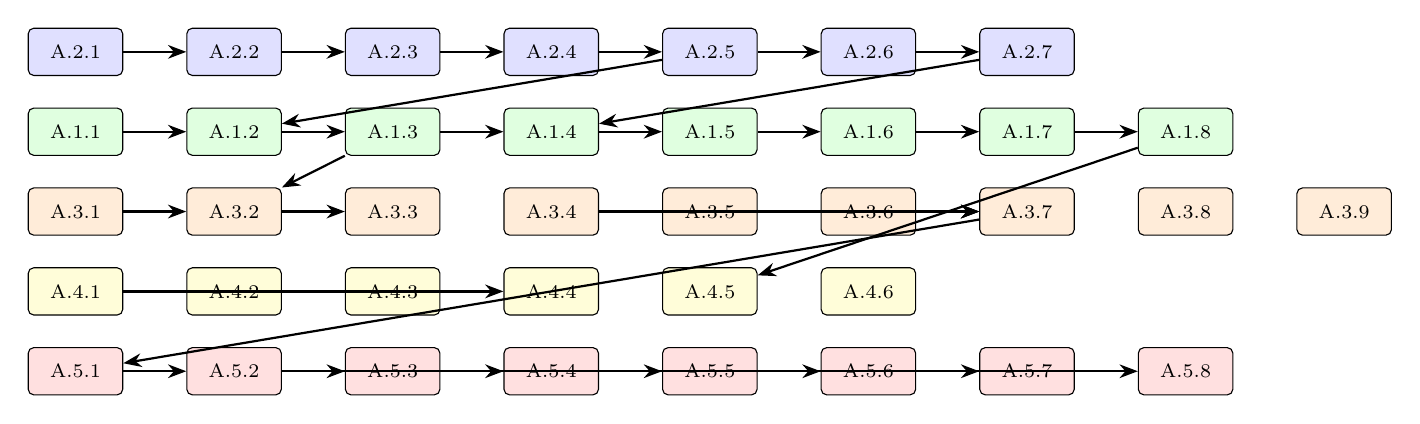
\begin{tikzpicture}[
  node distance=4mm and 8mm,
  every node/.style={font=\scriptsize},
  area/.style={draw, rounded corners=2pt, minimum height=6mm,
               minimum width=12mm},
  s/.style={area, fill=blue!12},
  r/.style={area, fill=green!12},
  cli/.style={area, fill=orange!15},
  tel/.style={area, fill=yellow!15},
  d/.style={area, fill=red!12},
  arr/.style={->, >=Stealth, thick}
]
% schemas critical path
\node[s] (a21) {A.2.1};
\node[s, right=of a21] (a22) {A.2.2};
\node[s, right=of a22] (a23) {A.2.3};
\node[s, right=of a23] (a24) {A.2.4};
\node[s, right=of a24] (a25) {A.2.5};
\node[s, right=of a25] (a26) {A.2.6};
\node[s, right=of a26] (a27) {A.2.7};
\foreach \i/\j in {a21/a22, a22/a23, a23/a24, a24/a25, a25/a26, a26/a27}
  \draw[arr] (\i) -- (\j);

% Supervisor core - depends on schemas
\node[r, below=of a21] (a11) {A.1.1};
\node[r, right=of a11] (a12) {A.1.2};
\node[r, right=of a12] (a13) {A.1.3};
\node[r, right=of a13] (a14) {A.1.4};
\node[r, right=of a14] (a15) {A.1.5};
\node[r, right=of a15] (a16) {A.1.6};
\node[r, right=of a16] (a17) {A.1.7};
\node[r, right=of a17] (a18) {A.1.8};
\foreach \i/\j in {a11/a12, a12/a13, a13/a14, a14/a15, a15/a16, a16/a17, a17/a18}
  \draw[arr] (\i) -- (\j);
\draw[arr] (a25) -- (a12);
\draw[arr] (a27) -- (a14);

% Runtime
\node[cli, below=of a11] (a31) {A.3.1};
\node[cli, right=of a31] (a32) {A.3.2};
\node[cli, right=of a32] (a33) {A.3.3};
\node[cli, right=of a33] (a34) {A.3.4};
\node[cli, right=of a34] (a35) {A.3.5};
\node[cli, right=of a35] (a36) {A.3.6};
\node[cli, right=of a36] (a37) {A.3.7};
\node[cli, right=of a37] (a38) {A.3.8};
\node[cli, right=of a38] (a39) {A.3.9};
\foreach \i/\j in {a31/a32, a32/a33, a34/a37, a35/a37, a36/a37}
  \draw[arr] (\i) -- (\j);
\draw[arr] (a13) -- (a32);

% Telemetry
\node[tel, below=of a31] (a41) {A.4.1};
\node[tel, right=of a41] (a42) {A.4.2};
\node[tel, right=of a42] (a43) {A.4.3};
\node[tel, right=of a43] (a44) {A.4.4};
\node[tel, right=of a44] (a45) {A.4.5};
\node[tel, right=of a45] (a46) {A.4.6};
\foreach \i/\j in {a41/a44, a18/a45}
  \draw[arr] (\i) -- (\j);

% Demo
\node[d, below=of a41] (a51) {A.5.1};
\node[d, right=of a51] (a52) {A.5.2};
\node[d, right=of a52] (a53) {A.5.3};
\node[d, right=of a53] (a54) {A.5.4};
\node[d, right=of a54] (a55) {A.5.5};
\node[d, right=of a55] (a56) {A.5.6};
\node[d, right=of a56] (a57) {A.5.7};
\node[d, right=of a57] (a58) {A.5.8};
\foreach \i/\j in {a51/a52, a52/a53, a52/a54, a52/a55, a52/a56, a56/a57, a52/a58}
  \draw[arr] (\i) -- (\j);
\draw[arr] (a37) -- (a51);
\end{tikzpicture}
\caption{The 38-task orchestration-layer development plan as a
dependency DAG. Blue = schemas (A.2); green = supervisor core (A.1);
orange = runtime (A.3); yellow = telemetry (A.4); red = demo (A.5).
The schemas critical path (top row) blocks every downstream sub-area;
A.5.6 (publishing \safelibyaml{} to crates.io) is the public-facing
deliverable.}
\label{fig:devplan-dag}
\end{figure}

% -------------------------------------------------------------------------
\subsection*{A.7 Two-week MVP Gantt}

\Cref{fig:devplan-gantt} renders the 38-task plan as a two-week Gantt
chart, assuming a three-engineer team with one tech lead. The schedule
shown is the \emph{aggressive} target derived directly from the per-task
hour estimates above; for calendar-time planning the team should apply a
1.5--2$\times$ multiplier (yielding a 3--4 week MVP) to absorb meeting
overhead, integration debugging, and review cycles. The critical path
runs through A.2 (schemas) on days 1--2, A.1 (supervisor core) on days
3--6, and A.5 (demo) on days 12--14, with A.3 (runtime) and A.4
(telemetry) overlapping on days 5--11.

\begin{figure}[h]
\centering
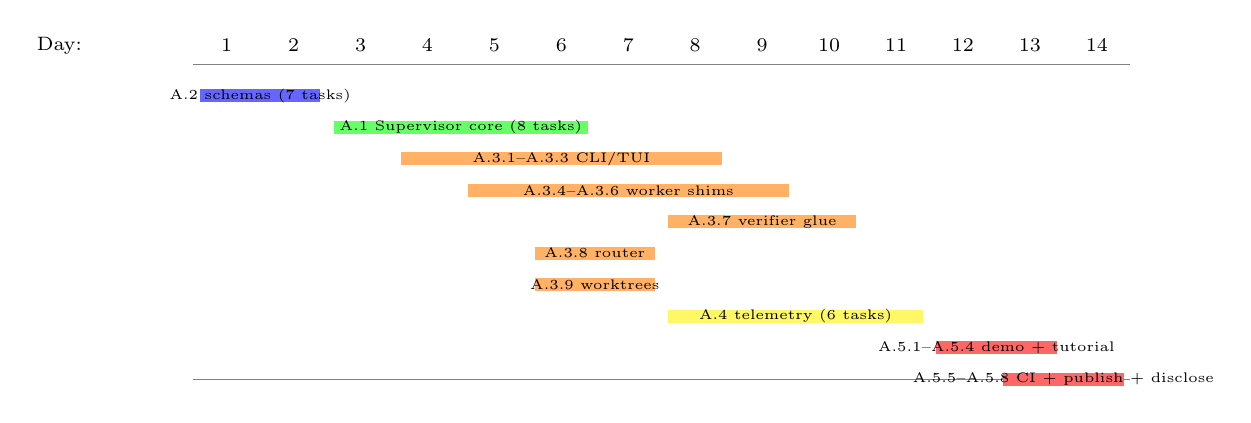
\begin{tikzpicture}[
  x=0.85cm, y=0.4cm,
  every node/.style={font=\scriptsize}
]
% axis
\foreach \d in {1,...,14} \node at (\d, 0.6) {\d};
\node at (-1.5, 0.6) {Day:};
\draw[thin, gray] (0.5, 0) -- (14.5, 0);
\draw[thin, gray] (0.5, -10) -- (14.5, -10);

\def\bar#1#2#3#4#5{%
  \fill[#5!60] (#1-0.4,-#3+0.2) rectangle (#2+0.4,-#3-0.2);
  \node at ({(#1+#2)/2}, -#3) {\tiny #4};
}

% schemas
\bar{1}{2}{1}{A.2 schemas (7 tasks)}{blue}
% Supervisor core
\bar{3}{6}{2}{A.1 Supervisor core (8 tasks)}{green}
% runtime
\bar{4}{8}{3}{A.3.1--A.3.3 CLI/TUI}{orange}
\bar{5}{9}{4}{A.3.4--A.3.6 worker shims}{orange}
\bar{8}{10}{5}{A.3.7 verifier glue}{orange}
\bar{6}{7}{6}{A.3.8 router}{orange}
\bar{6}{7}{7}{A.3.9 worktrees}{orange}
% telemetry
\bar{8}{11}{8}{A.4 telemetry (6 tasks)}{yellow}
% demo
\bar{12}{13}{9}{A.5.1--A.5.4 demo + tutorial}{red}
\bar{13}{14}{10}{A.5.5--A.5.8 CI + publish + disclose}{red}
\end{tikzpicture}
\caption{Two-week orchestration-layer MVP Gantt. Critical path
(top to bottom): A.2 schemas $\to$ A.1 Supervisor core $\to$ A.5 demo. The
runtime and telemetry tracks parallelise from day 4 onwards. The
deliverable on day 14 is a working \texttt{ferrous-bridge run --target
libyaml} CLI plus a published \safelibyaml{} 0.1.0 on
\texttt{crates.io}.}
\label{fig:devplan-gantt}
\end{figure}

\end{document}
